\documentclass[a4paper]{article}
\usepackage[T1]{fontenc}
\usepackage[utf8]{inputenc}
\usepackage[english]{babel}
\usepackage{graphicx}
\usepackage{float}
\usepackage{hyperref}
\usepackage{makeidx}
\usepackage{caption}
\usepackage{tabularx}
\usepackage[table, xcdraw, dvipsnames]{xcolor}

\graphicspath{ {images/} }
% !TeX spellcheck = en_US
\makeindex

\begin{document}
\title{TrackMe: Implementation document \\Software Engineer 2 - 2018/2019}
\author{
        Riccardo Poiani, Mattia Tibaldi, Tang-Tang Zhou \\
        Politecnico di Milano\\\\ 
        Version 1.0 \\
        \thanks{
		Link to source code:
        \url{https://github.com/tangtang95/PoianiTibaldiZhou/tree/master/Implementation}}
        \thanks{
	    Link to what has to be installed:
	    \url{https://github.com/tangtang95/PoianiTibaldiZhou/releases} and the software specified in the installation instruction.}
}
\maketitle
\newpage
\tableofcontents
\newpage

\section{Introduction}
The purpose of this document is to provide all the information regarding the implementation of a viable product of the TrackMe project: in
particular it regards the services of Data4Help and AutomatedSOS. 
It follows a brief description of the structure of the document:
\begin{itemize}
\item First of all, in the front page it is possible to find links to the source code and to what needs to be installed
\item The second section illustrates what are the requirements that have been actually implemented, providing some useful motivations
in order to understand the choices that were made 
\item The third one takes into consideration the frameworks adopted, recapping and introducing further comments on what was already
mentioned in the Design Document. Moreover, benefits and drawbacks are better analyzed, and ulterior decisions are discussed
\item The fourth chapter analyzes the structure of the source code and diagrams are presented to illustrate a precise structure of
the written code 
\item The fifth section provides information on how tests were written. Coverage is here presented and system tests is presented and commented
\item The final chapter helps in understanding what is necessary to do in order to install and run the software, with all the necessary prerequisites 
\end{itemize}


\documentclass[a4paper]{article}
\usepackage[T1]{fontenc}
\usepackage[utf8]{inputenc}
\usepackage[english]{babel}
\usepackage{graphicx}
\usepackage{float}
\usepackage{hyperref}
\usepackage{makeidx}
\usepackage{caption}
\usepackage{tabularx}
\usepackage[table, xcdraw, dvipsnames]{xcolor}

\graphicspath{ {images/} }
% !TeX spellcheck = en_US
\makeindex

\begin{document}
\title{TrackMe: DD \\Software Engineer 2 - 2018/2019}
\author{
        Riccardo Poiani, Mattia Tibaldi, Tang-Tang Zhou \\
        Politecnico di Milano\\\\ 
        Version 1.0
}
\maketitle
\newpage
\tableofcontents
\newpage

\section{Introduction}
The purpose of this document is to provide all the information regarding the implementation of a viable product of the TrackMe project: in
particular it regards the services of Data4Help and AutomatedSOS. 
It follows a brief description of the structure of the document:
\begin{itemize}
\item First of all, in the front page it is possible to find links to the source code and to what needs to be installed
\item The second section illustrates what are the requirements that have been actually implemented, providing some useful motivations
in order to understand the choices that were made 
\item The third one takes into consideration the frameworks adopted, recapping and introducing further comments on what was already
mentioned in the Design Document. Moreover, benefits and drawbacks are better analyzed, and ulterior decisions are discussed
\item The fourth chapter analyzes the structure of the source code and diagrams are presented to illustrate a precise structure of
the written code 
\item The fifth section provides information on how tests were written. Coverage is here presented and system tests is presented and commented
\item The final chapter helps in understanding what is necessary to do in order to install and run the software, with all the necessary prerequisites 
\end{itemize}


\newpage

\section{Architecture Design}
\subsection{Overview}
In this whole chapter the architecture design process is described, and it contains all the significant
architecture decisions. 
Therefore, first of all, in this section a high-level and very general architecture for the TrackMe 
project is presented and discussed.  

\begin{figure}[H]
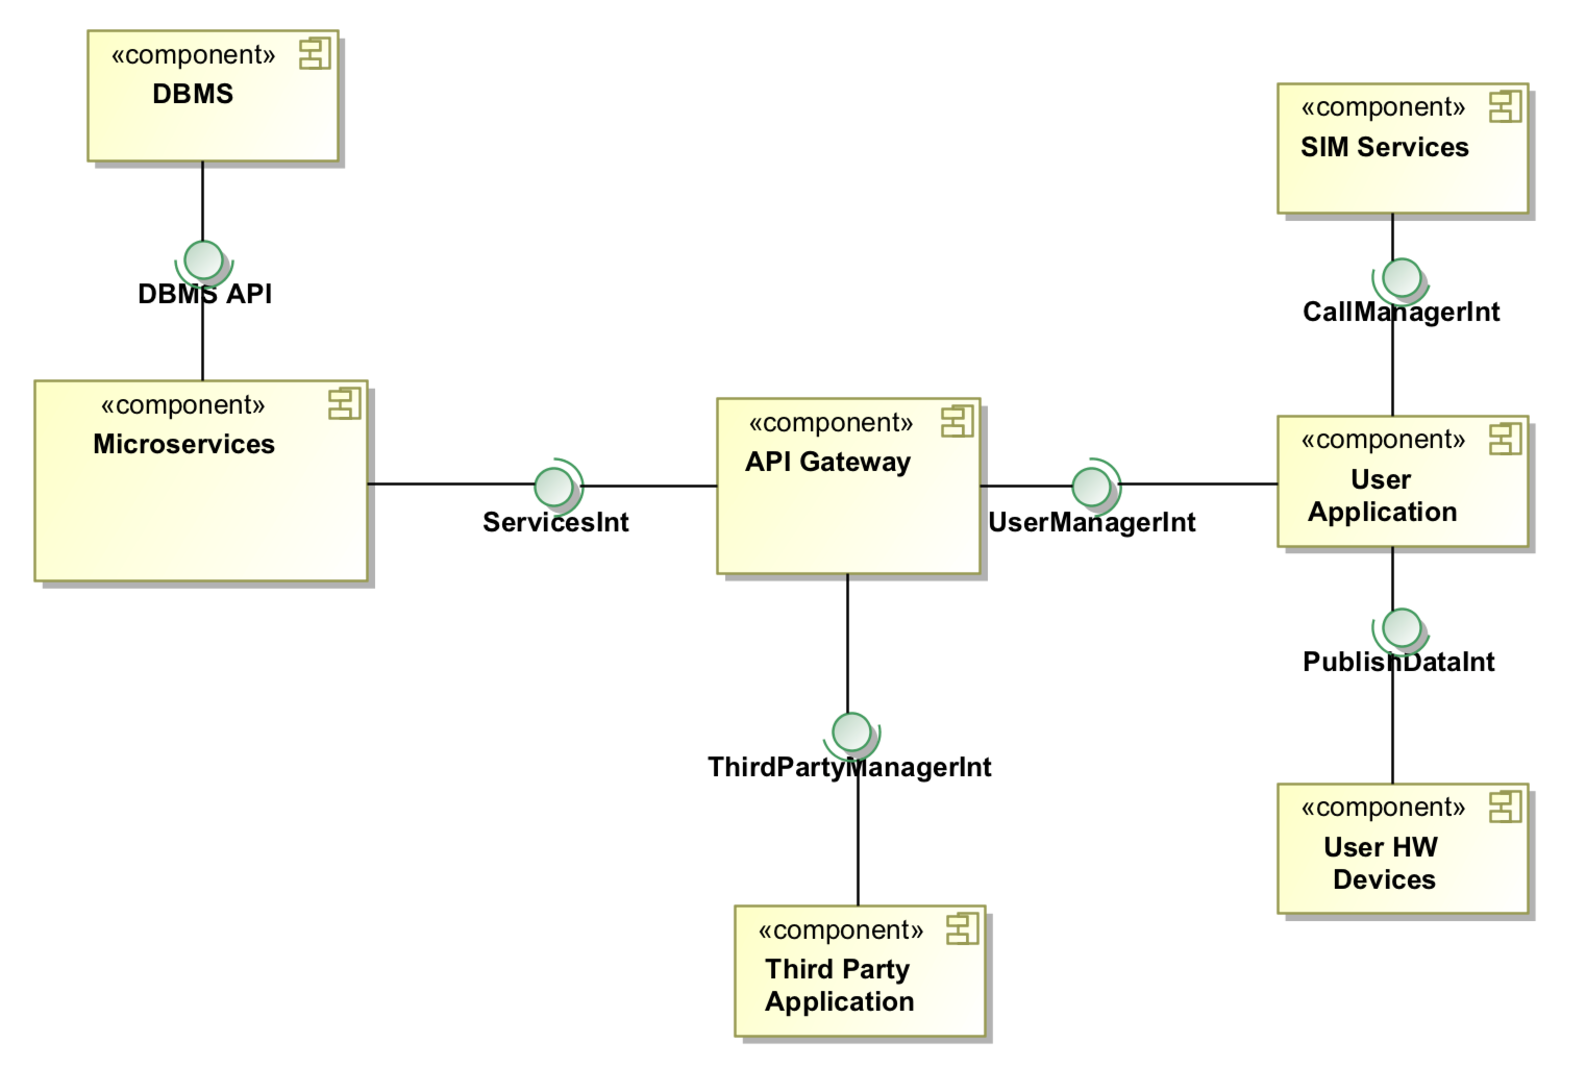
\includegraphics[width=\linewidth]{Images/highlevelcd.pdf}
\caption{ High-level component diagram }
\label{fig:highlevelcomponentdiagram}
\end{figure}

As a reference architecture, the microservices one has been considered: this decision will be later discussed. \\
From the picture, it is evident that the clients can access the services by means of an API gateway, that will provide authentication 
to the users, and forwards the requests to the correct microservices based on the service registry.
Of course, a new service instance needs to register to the service registry in order to be located by the API gateway. \\
Another relevant information is that the project can be ideally split, at a high level, into two applications: one for the users and one for the third parties customers: they both interact with the API gateway, that will guarantee to access all the
microservices that compose the core functionality of the business.
More specifically, the "microservices" block includes Data4Help and Track4Run functions, while the goals
of AutomatedSOS service are reached locally and directly by means of the user application, that, when
needed, will perform a call with the help of the SIM service. 
The user application also needs to communicate with a device that is able to collect data regarding his health: more specifically, this
instrument will send data toward the user application autonomously, without being asked.
Examples of  this machines are smartrings and smartwatches. 
The data regarding the position of the user is, instead, retrieved via GPS's API. \\
Note, also, that the microservices need to keep some data persistent, and, thus access to a DBMS, by means
of its API. 
Moreover, some services need also to communicate and share information: this is achieved via the message queue, that is
charged of receiving and forwarding messages to the interested parts. \\


\subsection{Component view}
In this section, components are expanded and better analyzed. \\
The main analysis regards the microservices block: 
\begin{figure}[H]
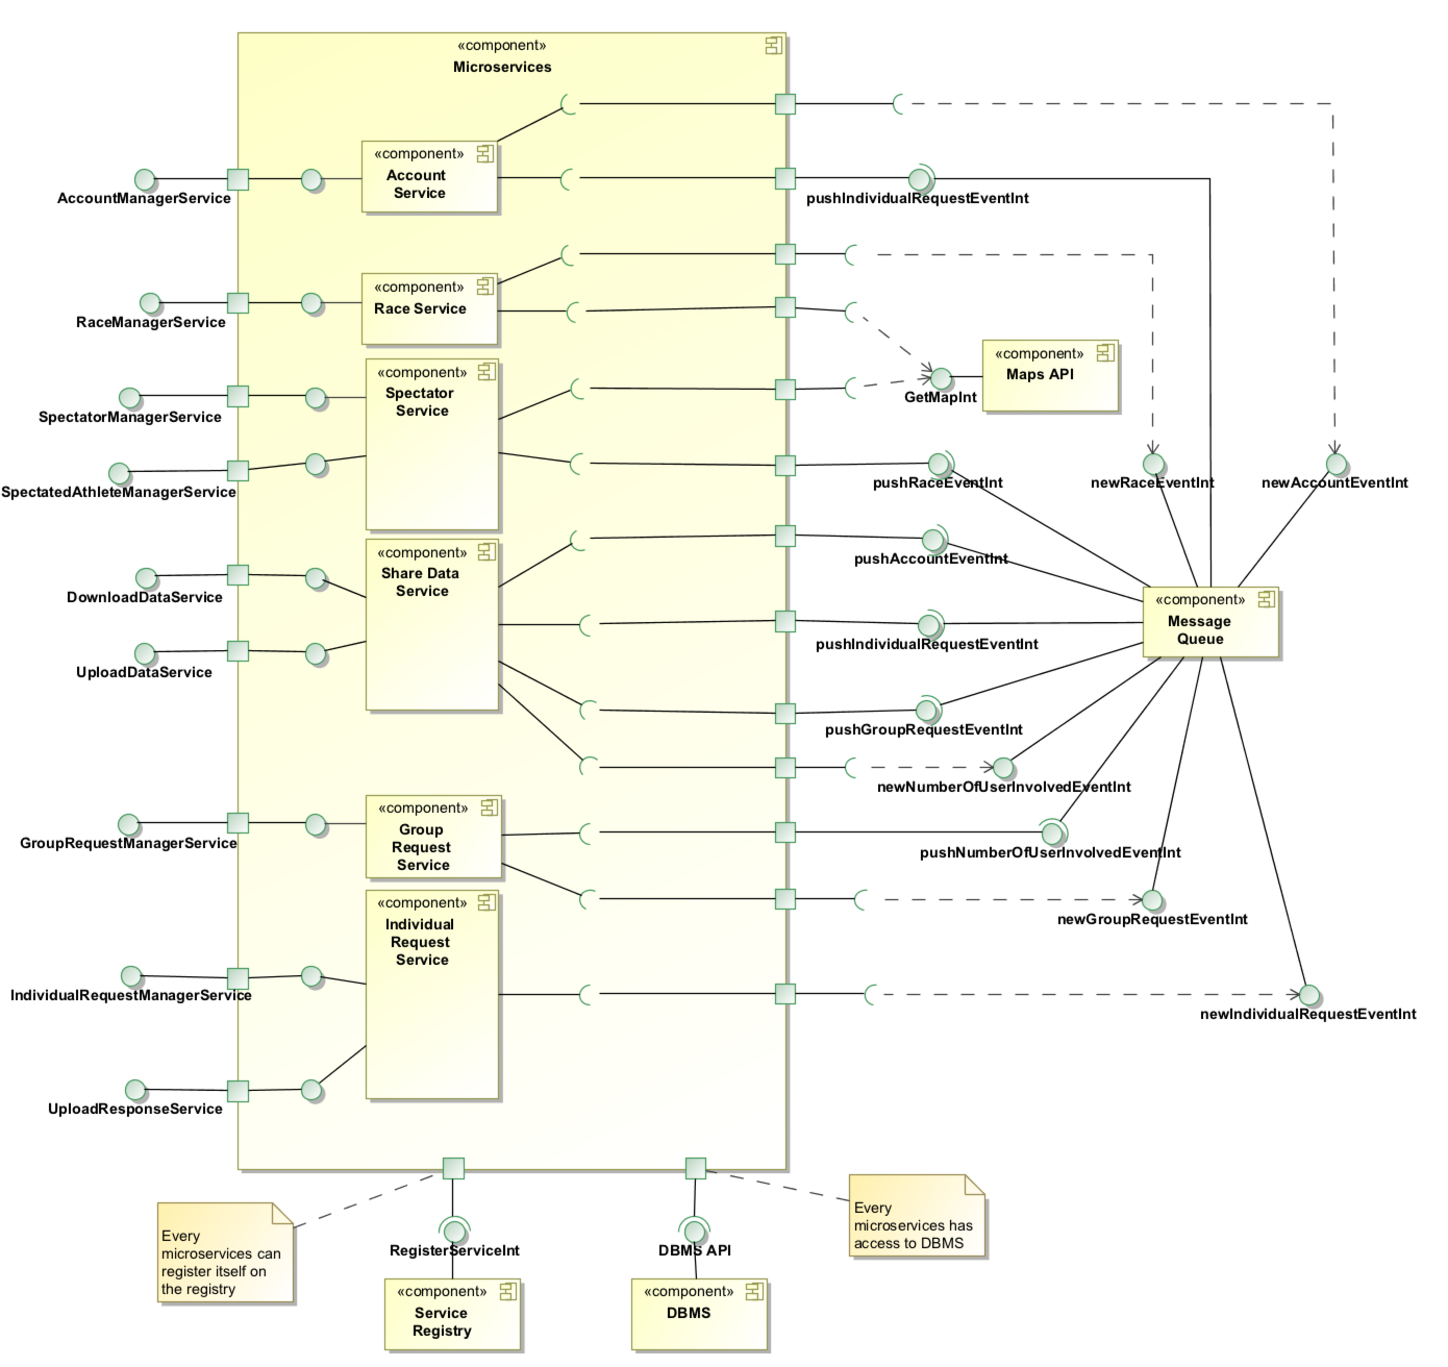
\includegraphics[width=\linewidth]{Images/componentdiagram.pdf}
\caption{ Component diagram }
\label{fig:componentdiagram}
\end{figure}
Various service components are present, and they all expose at least an interface that is accessed by the
clients via the joint combination of API gateway and router.
It follows a brief description of the various services, and a better specification of the interfaces they provide to users and third party customers:
\begin{itemize}
\item The account service provides all the functions related to user sessions, such as login and logout,
and also the registration of clients 
\item The race service makes possible for an athlete to enroll in a run; for a third party customer to set
up one, and also close it; and it also enables the possibility of retrieving the available races and their
status (e.g. in course, terminated). Therefore, it manages the "more static" part
of a race
\item The spectator service regards the dynamic part of a race, such as the fact that a user can spectate
athletes who are running (therefore they can retrieve their positions and the leaderboard). This
service is also in charge of receiving position data of the participants
\item Share data service is responsible for the monitoring the user health statuses and positions: here a
user will upload his data. Furthermore, third party customer will access the data that they have
previously requested, by means of "AccessDataService" interface
\item The group request service provides to the third parties the possibility of uploading group requests and see their status 
\item The individual request service enables third party customer to upload individual request and monitor their status, and allows a user to
check if there are some requests for him, and, eventually, upload responses 
\end{itemize}

Microservices have their own data and, therefore, access DBMS's API, while Maps's API are necessary 
only for race and spectator service, in order to manage and double check position data and feasible paths. \\
The diagram also shows the main communications that take place between components. 
The following message exchange is needed to completely and correctly exploit the project functions. 
\begin{itemize}
\item 
When a third party is accessing individual data through the data share service, it
needs to know if a request associated with those data was sent and accepted. 
Indeed, the request acceptance and its data, are managed in the following way: when an individual request has been accepted, a message is sent through the message queue with the help of an interface, IndividualRequestEventPublisher. Then, this message reaches the share data service thanks to the interface provided by it (i.e. IndividualRequestEventListener). \\
Moreover, to guarantee that individual requests must be performed on registered users, a match with the account service 
is necessary. When a new user registers, the account service will send the data about the user through the message queue to reach 
all the services which need it. One of these services is the Individual Request Service which needs the user to check if an individual 
request is coherent with the system (UserEventListener and UserEventPublisher are the interfaces that accomplish this task). 
\item 
A slightly different reasoning holds for the management of the group requests. In this case, the exchange is bidirectional. 
In particular, when a new group request is performed, the share data service will be notified by the message queue via the
GroupRequestEventListener, and it will be sent to the message queue by GroupRequestEventPublisher. \\
When the share data service receives this event, it will query its data in order to retrieve information regarding the number of users
involved: of course, this information needs to be sent back to the group request service, that will accept or refuse the request
(DataEventListener and DataEventPublisher are the interfaces that accomplish this task). 
Of course, the acceptance of the request may trigger again the new group request event. 
However, this will be later exposed and commented in the run time view. \\
Moreover, to guarantee that the filters on the aggregated request are applied correctly (e.g. data on the users whose age is greater then 40)
a match with the account service is needed. 
Indeed, when a user registers to the service, the account service will sends user information to the message queue with UserEventPublisher. 
The information will be forwarded to the share data service with UserEventListener.
\item
Another important message exchange is between spectator and race services: in particular, data that the spectator service is receiving must
be matched with an active run, and thus it needs to know the status of the run: the changes will be communicated by 
RaceEventListener and RaceEventPublisher.
\end{itemize}

\subsection{Deployment view}
\par
Regarding the deployment, there are many quality to take into consideration. One of these is the scalability property: at the beginning 
TrackMe might only have few users, but once the usage is increasing more and more, the system must continue to work even if the 
requests from the users are huge. To achieve this quality of service, TrackMe needs the help of cloud database providers. These ones 
are specialized in the management of big database; and in this case the Share Data Service require a huge database in order to store 
all the data collected from the users. 
\par
On the other side, services such as Account Service, Individual Request Service and Group Request Service do not require so much 
power. Therefore, a good solution is the virtualization; in such a way each microservices has its own application server, while 
the database server can be shared among these services.. Instead, Spectator Service require to save a good amount of data and 
the access might be frequent due to the requirement regarding the possibility to see all the positions of the runners during a race. 
Consequently, Spectator Service has its own database 
server machine.
\par
To access these microservices one needs to use the mobile application which has to be installed either on an Android device or on a iOS 
device; Firewalls are used to separate the client domain and the server domain, and also used to filter packets which can be malevolent.
\begin{figure}[H]
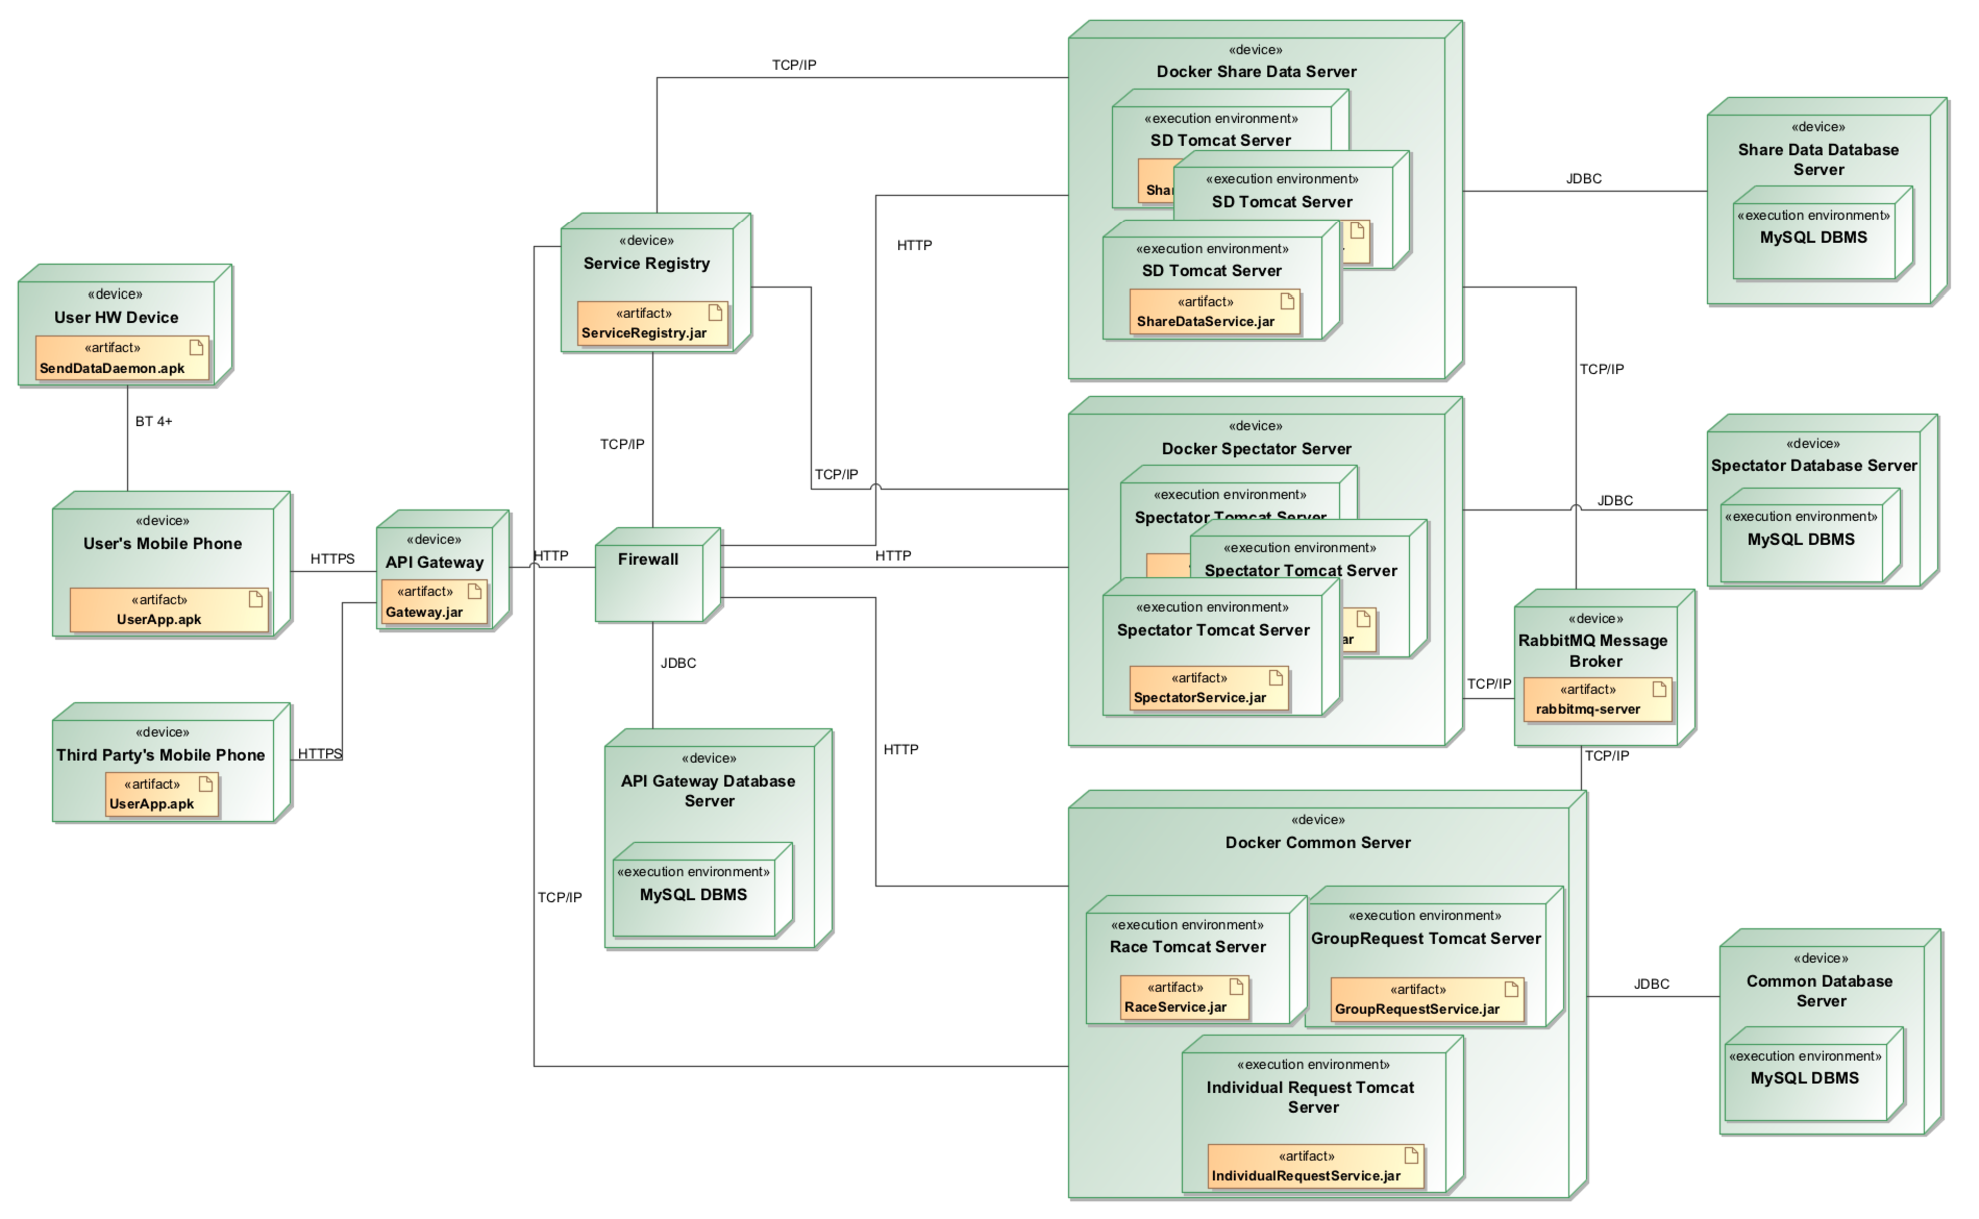
\includegraphics[width=\linewidth]{Images/deploymentdiagram.pdf}
\caption{ Deployment diagram with Archimate }
\label{fig:deployment}
\end{figure}
The deployment diagram represents the system to-be which is based on the microservices "reference architecture". Even if 
microservices offer the possibility to implement different services with different programming language or framework, what is simpler 
is to keep using the same environment. In this case, Glassfish application server and Oracle DBMS are strongly used. In conclusion, 
the system can be also seen as clients and many servers with 4 tier:
\begin{itemize}
\item Tier 1: Client side, which is the presentation
\item Tier 2: API Gateway, which redirects all the requests from the client to the respective application server
\item Tier 3: Application servers, which contains the logic business of the system
\item Tier 4: Database servers, in which it contains all the data
\end{itemize}
\subsection{Runtime view}

\subsection{Component interfaces}
Here follows the interfaces of the various components that are available. 
Note that interfaces of external components (e.g. DBMS's API, CallManagerInt, GPSInt, MapsAPI) are not present. 

\begin{figure}[H]
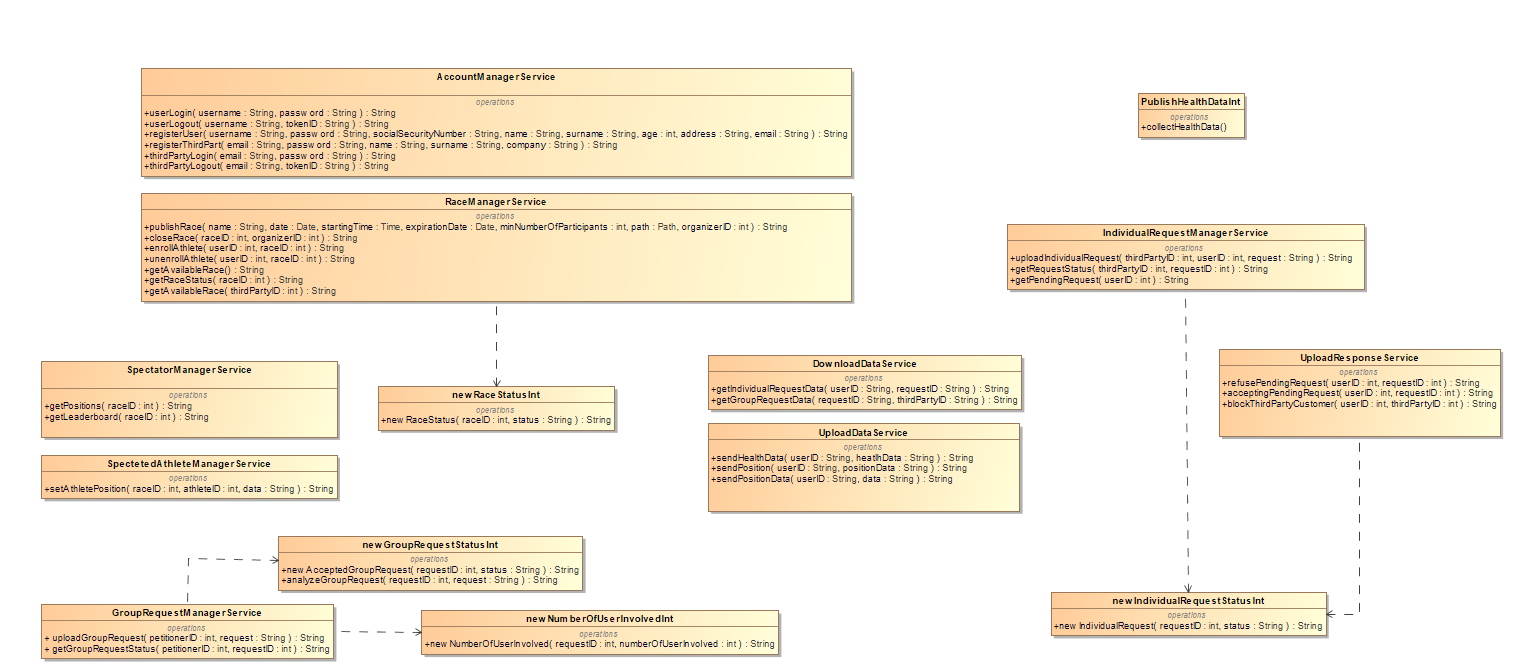
\includegraphics[width=\linewidth]{Images/componentinterfaces.png}
\caption{ Component interfaces }
\label{fig:componentinterface}
\end{figure}

In order to simplify the diagram, the API gateway has been excluded, but what it exposes is just the following: it provides a link for each
interface that is external w.r.t. the microservices block in figure \ref{fig:componentdiagram}. However, there is a little modification in the
parameters requested: indeed, the id of the client that is requesting the service (e.g. userID, thirdPartyID, athleteID) is substituted with
tokenID, in order to manage the authentication. This holds, clearly, with the exception of the registration and login feature, since a token 
is not available at this early stage of the user session. \\ 
A same reasoning is applied for what concerns the router: it just forwards the "translated" requests.
\subsection{Selected architectural styles and patterns}
In this section, all the adopted architectural styles and patterns are explained sufficiently to define why the specific style or pattern is chosen.

\subsubsection{Microservices}
The selected architectural style, as already mentioned, is the microservices architecture. This choice is
supported by multiple reasons. In particular, a strong motivation in the decision process is the
conjunction of the following two facts:
\begin{enumerate}
\item Data4Help and Track4Run are features that provides totally different and independent functions.
Track4Run can, without any problem, even be deployed in a different moment
\item Scalability is one of the main QoS that the system requires. Indeed, the application is expected to
be used by many people in the future, and therefore, designing the architecture making scaling fast is
really important
\end{enumerate}
It is important to note that it could happen that one of the two functions needs to scale, while
the other does not. 
More specifically, this reasoning also applies to some pieces of functionality that
are internal to both Data4Help and Track4Run. 
For instance, it is reasonable to assume that the functions of data collection from users (positions and
health statuses) will be much more used and will generate much more network traffic, compared to the one
that regards the requests. 
In order to clarify this, all the active users will periodically send data at each moment of the day,
while third party customers that are performing requests do not keep forwarding request to the user: it is
something that happens more rarely. 
The same holds, for example, when considering the set up of run events from the organizer, and the fact
that spectators will monitor in real time positions of athletes during a race. \\ 
Therefore, the combination of these things, suggests that the scaling should be independent w.r.t. the
function considered. \\
Furthermore, the microservices architecture makes it easier to implement failure isolation: it is not
desirable that a failure in Track4Run leads in a failure in also Data4Help. 
Moreover, failing in managing the request should not prevent the data collection: as one can see the
reason also applies to the various business capabilities that are bounded in the single Data4Help, or
Track4Run, feature.  
Due to this, the overall availability is improved. 

\subsubsection{Eventually consistency and compensation}
Before going to analyze all the patterns adopted for the microservices architecture, one must define the most important thing in a microservices architecture: how to achieve consistency of data. For instance, solutions for this issue are:
\begin{itemize}
\item Avoiding transactions across microservices: usually if a microservices architecture needs to have distributed transactions 
it means that there are redundant data. But if this is avoided, the lack of redundant data means that everytime a microservice needs 
to ask data from another microservice, a request is sent and if the other microservice is under high load, it will not be able to 
process it fast.
\item Two-Phase commit protocol (2PC): The distributed transaction of 2PC consists on two steps: Prepare phase (lock-phase) 
and Commit-rollback phase (unlock-phase). The problem with this protocol is that it is too slow compared to the time for an 
operation of a single microservice.
\item Eventual consistency and compensation: it is a model different from ACID transactions, but it is a mechanism to 
achieve consistency eventually at some point in the future. This might not achieve the same thing as 2PC but it is faster and if 
the architecture does not need the strict properties of ACID, then it is better. Otherwise, it could be very difficult to implement it.
\end{itemize}
Out of the three solutions, 2PC is not an option since the messages are synchronous, which means too slow. Therefore, Eventual consistency and compensation is the one adopted by this project due to the fact that the system will scale a lot and there is no problem if consistency is achieved in the future.


\subsubsection{Design patterns}
Now, some patterns adopted related to the microservices architecture are exposed:
\begin{itemize}
\item API gateway: this is a component already introduced in the high level component diagram and it
satisfies and deals with the following problem: how do clients of the application access to the individual
services? The API gateway is a single entry point for all clients and it can expose different API for
each client: this suits well for the TrackMe project. This should be implemented with an event-driven
reactive approach in order to scale if it is necessary to manage big loads of data \\
\item The access token pattern is very useful, since the application is composed of various services and
an important issue is how to communicate the identity of the petitioner to the service that handles the
request. 
The pattern suggests to implement the API gateway in such
a way that it authenticates requests and passes an access token that securely identifies the client (a
service may later include the access token in requests that it makes to other services)
\item Database per service pattern: all the services need to persist data in some kind of databases and
the solution is to keep each microservice's data private to that service and accessible only via its API.
So a database can't be accessed directly by another service. In particular the pattern of schema-per
service is always guaranteed, while a database-server-per-service is allocated to the services that are
though to be the one with the highest throughput (i.e. spectator service and share data service)
\item The messages and the communications between services, that were already introduced in the component diagram, are implement by means of
asynchronous messages, since a chain of synchronous calls could lead to slowdown the entire architecture. Note, that this leads to the
replication of some data, however, performance is considered more important than cost in this case. A way to achieve a better communications between services is to use something similar to the API gateway: a message queue architecture which requires also an additional service called message broker that is responsible for gathering, routing and distributing messages from services to other services (something similar to a mail service)
\item 
As shown, services need to call one another, but a microservices-based application typically runs in a virtualized 
environment where the number of instances of a service and their locations changes dynamically. 
The solution is to use a router that runs at a well known location. 
The router will query a service registry, which may be built into the
router, and forwards the requests to an available service instance.
Of course, when a new instance is created, it has to perform registration to the service registry. \\
The API gateway will send translated requests to the router, that will load balance them onto the active instances.
This pattern gives great benefits: indeed, the clients do not deal with the discovery of the service, but it comes with the drawback of
an additional component that need to be installed and configured, and, if needed, replicated, in order to scale
\item Microservices expose REST API that will be provided only by HTTPS endpoints. This will ensure
all the benefits of REST API, such the fact that services are stateless, with the security of an high-level encryption protocol. Other
benefits of the REST API which are relevant to the requirements of the project are: separation of concerns between client and server, reliability and scalability.
\item Saga pattern: this design pattern is, practically, a way to achieve the solution of Eventual consistency and compensation described before. It solves the trouble of distributed transactions without using 2PC by using a sequence of local transactions where each transaction updates data within a single service. Even though 2PC guarantees ACID properties, it is better Saga pattern that achieves only different properties, called BASE: Basic Availability Soft-state Eventually consistent.  But with Saga, there are two main different ways to implement a saga transaction:
\begin{itemize}
\item Events/Choreography: each service subscribes and publishes to other service's events
\item Command/Orchestration: there is a central coordinator service which is responsible about decision making and sequencing business logic 
\end{itemize}
In the project it is implemented the version of event transaction. Other than this implementation, Saga pattern defines also 
the compensation action: an action to restore the original states if there are failures during a distributed transaction (e.g. in 
the individual request service, if a third party sends a request regarding a non-existing social security number, then when 
account service is triggered, it will send a compensation action to the individual request by saying that the request must be canceled).

\end{itemize}
\subsection{Other design decisions}
\subsubsection{Frameworks}
The chosen and described architectural style, leads to some choices in the framework that will be used for the development and the deployment. 
In particular, to implement a microservices architecture, a microservices chassis framework is needed, in order to have the best support 
in the developing phase. 
An option here is to adopt both Spring Boot (for what concerns the microservices) and Spring Cloud (that facilitates the set up of distributed
system software). They are widely adopted and greatly supported by the community; also many guides and articles are available on the internet. \\

\subsubsection{Asynchronous messages}
RabbitMQ, that is a message broker server, is used to implement the exchange of messages among services. This choice is motivated 
by the following facts: it enhances delivery and order guarantee, redundancy, decoupling and scalability. 
Finally, it is well supported in Spring boot. 

\subsubsection{Data transfer encryption}
Another important issue is regarding the communication between the user hardware device and the user application. This is encrypted with
AES-128. \\
The communication happens by means of bluetooth: the version 4.0 + LE, that is available from 2010, provides some nice features for the
project, because it grants enough bandwidth (1Mbps when the low energy mode is enabled) for transmitting the data, and it is also a low
energy consumer. Furthermore, there is no need of internet connection (with the limits of the network coverage): the devices just need to be
close, but this is a totally rational assumption, given the context of the application. 
Note that this version ensures a good compatibility with a large set of devices. 

\subsubsection{Android application} 	 
The user application will be developed for the Android operative system, at least in a first moment. This is due to the criticality of the
automatedSOS service. Assuming that the application will be deployed with Italy as the first market target, this choice covers the biggest
part of the market.

\subsubsection{JSON}
REST API will be implemented using JSON as a protocol for exchanging data. \\
Compared to XML, it is less verbose and JSON packets require less size. Furthermore, it is well supported
by Spring Boot. 

\subsubsection{Group Request Filtering}
Up until now, group requests were more or less abstract: there was no definition of what group requests could possibly get from 
data. Therefore, here it is defined what group requests return. The only outcomes they give are  aggregated data, i.e. count 
of tuples, sum of values, average of values or other aggregate operator available (e.g. in SQL). Another thing to clarify is that 
the tuples of the result from a group request have to satisfy a certain constraint requested by the petitioner. Consequently, 
the following filters are the ones available:
\begin{itemize}
\item Filtering by birth city
\item Filtering by birth nation
\item Filtering by birth year
\item Filtering by the GPS position data
\item Filtering by the health statuses
\item Filtering by date and time
\end{itemize}
Since this type of service is very difficult to implement for the user (user-friendly difficult), each filter is applied to decrease the number of users and every query is applied only to users that have at least one position data and one health data. Basically there is no group-by statement in the query.







\newpage

\section{User interface design}


\newpage

\section{Requirements traceability}
Below are listed the design components to which Data4Help requirements and goals are mapped: 
\begin{itemize}
\item[{[G1]}] Allow a user to access its own data. Requirements([R10])
	\begin{enumerate}
	\item Account service.
	\item Share data service.
	\end{enumerate}
\item[{[G2]}] Allow a user to contribute to data sharing by providing information about his location and health status. Requirements([R11])
	\begin{enumerate}
	\item Share data service.
	\end{enumerate}
\item[{[G3 \& G4]}] Once the health parameters of a user have been observed below the threshold for the first time after one hour, an ambulance is sent to the user location. 
The time experienced between the moment in which the health parameters of a subscribed user are observed below the threshold and the time in which the emergency point is contacted is equal or less than 5 seconds. Requirements([R12]-[R13]-[R14]-[R14]-[R15]-[R16]-[R17])
	\begin{enumerate}
	\item Share data service.
	\item SIM services.
	\end{enumerate}
\item[{[G5]}] Allow a user to participate in a run managed by third parties, as an athlete, if all starting conditions are satisfied. Requirements([R18]-[R19]-[R20]-[R21]-[R22])
	\begin{enumerate}
	\item Race service.
	\end{enumerate}
\item[{[G6]}] Allow spectators (i.e. user) to see on real-time the "correct" positions of all athletes taking part in a run, with at most 15 meters of radius error.
Requirements([R23]-[R24])
	\begin{enumerate}
	\item  Spectator service.
	\end{enumerate}
\item[{[G7]}] The maximum time to accept an individual request from any third party is 30 days; after that, the request will expire. Requirements([R25])
	\begin{enumerate}
	\item Individual request service.
	\item Group request service.
	\end{enumerate}
\item[{[G8 \& G9]}] Allow a user to accept or refuse a request from third parties. Allow a user to block requests made by a specific third party. Requirements([R26]-[R27]-[R28]-[R29])
	\begin{enumerate}
	\item Individual request service.
	\end{enumerate}
\item[{[G10]}] Allow spectators and runners to see the leader board, when a run is completed. Requirements([R30]-[R31]-[R32])
	\begin{enumerate}
	\item Spectator service.
	\end{enumerate}
\item[{[G11]}] Allow organizers (i.e. third parties) to set up a run, by defining its name, its path, date, start time, expiration date, and the minimum number of participants. Requirements([R33]-[R34])
	\begin{enumerate}
	\item Race service.
	\end{enumerate}
\item[{[G12]}] Allow a third party to access data specified in a request if the user accepts the request or if he accepted one or more requests from the same third party that provided access to the same data. Requirements([R35]-[R36]-[R37]-[R38])
	\begin{enumerate}
	\item Individual request service.
	\end{enumerate}
\item[{[G13]}] Allow a third party to access statistical and anonymized data if and only if the number of individual involved is greater than 1000. This is satisfied as soon as the request is approved. Requirements([R39]-[R40]-[R41]-[R42])
	\begin{enumerate}
	\item Group request service.
	\end{enumerate}
\item[{[G14]}] Allow a third party to subscribe to non-existing data. They will have access to them, as soon as the data is generated. Requirements([R43]-[R44])
	\begin{enumerate}
	\item Individual request service.
	\item Group request service.
	\end{enumerate}
\end{itemize}

\newpage

\section{Implementation, integration and test plan}

\newpage

\section{Effort Spent}

\subsection{Riccardo Poiani}

\begin{table}[H]
\begin{tabularx}{\textwidth}{|l|X|c|}
\hline
\rowcolor[HTML]{C0C0C0} 
Date & Task & Hours\\ \hline
15/10 & Goal definitions & 2.5\\ \hline
17/10 & Document structure, goal definition, class diagram & 2.5\\ \hline
18/10 & state diagram, class diagram, purpose, hypothesis & 1.5\\ \hline
19/10 & Scope, purpose and state diagram & 2\\ \hline
22/10 & Product functions & 2\\ \hline
23/10 & Scenarios & 2\\ \hline
24/10 & Scenarios & 1\\ \hline
25/10 & Refactor all document (revising) & 1\\ \hline
26/10 & Refactor all document (revising) & 4\\ \hline
27/10 & Add design standards, performance, availability, reliability, security; Add use case diagram and sequence diagram & 5\\ \hline
27/10 & Alloy & 2\\ \hline
28/10 & Alloy; world and shared phenomena; use case; whole document revision; sequence diagram & 7.5  \\ \hline
29/10 & Alloy; sequence diagram; fix requirement& 3 \\ \hline
01/11 & Revise document & 4 \\ \hline 
\rowcolor[HTML]{C0C0C0} 
& Overall & 40 \\ \hline
\end{tabularx}
\end{table}

\subsection{Mattia Tibaldi}

\begin{table}[H]
\begin{tabularx}{\textwidth}{|l|X|c|}
\hline
\rowcolor[HTML]{C0C0C0} 
Date & Task & Hours\\ \hline
15/10 & Goal definitions & 1.5\\ \hline
17/10 & Introduction & 2\\ \hline
18/10 & Scope and purpose & 4\\ \hline
19/10 & State diagram & 1\\ \hline
22/10 & Hardware interfaces & 2\\ \hline 
23/10 & Software interfaces & 3.5\\ \hline
24/10 & User interfaces & 3\\ \hline
25/10 & User interfaces and communication interfaces & 4\\ \hline 
27/10 & Revise document and use case & 3.5\\ \hline
28/10 & Alloy & 4.5\\ \hline
29/10 & Alloy and refactor document & 4\\ \hline
01/11 & Revise document & 4 \\ \hline 
\rowcolor[HTML]{C0C0C0} 
& Overall & 36\\ \hline
\end{tabularx}
\end{table}

\subsection{Tang-Tang Zhou}

\begin{table}[H]
\begin{tabularx}{\textwidth}{|l|X|c|}
\hline
\rowcolor[HTML]{C0C0C0} 
Date & Task & Hours\\ \hline
15/10 & Goal definitions & 2.5\\ \hline
17/10 & Document structure, goal definition, class diagram & 2.5\\ \hline
18/10 & state diagram, class diagram, purpose, hypothesis & 1.5\\ \hline
20/10 & Product Perspective, race diagram, request diagram and Alloy & 4\\ \hline
21/10 & Alloy & 1.5 \\ \hline
22/10 & Fix goals, purpose and perspective & 2\\ \hline
23/10 & Domain asssumptions and requirements & 2\\ \hline
24/10 & Requirements, goals, assumptions & 2\\ \hline
25/10 & Refactor all document (revising) & 2\\ \hline
26/10 & Refactor all document (revising) & 3\\ \hline
27/10 & Fix requirements, add alloy, add use case and sequence diagram & 5\\ \hline
27/10 & Add mantainability, portability, definitions, structure and references & 2\\ \hline
28/10 & Revise document, fix diagrams, add sequence diagram to document, add effort spent & 5\\ \hline
29/10 & Fix diagrams, Add alloy worlds, fix requirements & 2 \\ \hline
31/10 & sequence diagram & 1 \\ \hline
01/11 & Revise document & 3 \\ \hline 
\rowcolor[HTML]{C0C0C0} 
& Overall & 41\\ \hline
\end{tabularx}
\end{table}

\newpage

\end{document}


\documentclass[a4paper]{article}
\usepackage[T1]{fontenc}
\usepackage[utf8]{inputenc}
\usepackage[english]{babel}
\usepackage{graphicx}
\usepackage{float}
\usepackage{hyperref}
\usepackage{makeidx}
\usepackage{caption}
\usepackage{tabularx}
\usepackage[table, xcdraw, dvipsnames]{xcolor}

\graphicspath{ {images/} }
% !TeX spellcheck = en_US
\makeindex

\begin{document}
\title{TrackMe: DD \\Software Engineer 2 - 2018/2019}
\author{
        Riccardo Poiani, Mattia Tibaldi, Tang-Tang Zhou \\
        Politecnico di Milano\\\\ 
        Version 1.0
}
\maketitle
\newpage
\tableofcontents
\newpage

\section{Introduction}
The purpose of this document is to provide all the information regarding the implementation of a viable product of the TrackMe project: in
particular it regards the services of Data4Help and AutomatedSOS. 
It follows a brief description of the structure of the document:
\begin{itemize}
\item First of all, in the front page it is possible to find links to the source code and to what needs to be installed
\item The second section illustrates what are the requirements that have been actually implemented, providing some useful motivations
in order to understand the choices that were made 
\item The third one takes into consideration the frameworks adopted, recapping and introducing further comments on what was already
mentioned in the Design Document. Moreover, benefits and drawbacks are better analyzed, and ulterior decisions are discussed
\item The fourth chapter analyzes the structure of the source code and diagrams are presented to illustrate a precise structure of
the written code 
\item The fifth section provides information on how tests were written. Coverage is here presented and system tests is presented and commented
\item The final chapter helps in understanding what is necessary to do in order to install and run the software, with all the necessary prerequisites 
\end{itemize}


\newpage

\section{Architecture Design}
\subsection{Overview}
In this whole chapter the architecture design process is described, and it contains all the significant
architecture decisions. 
Therefore, first of all, in this section a high-level and very general architecture for the TrackMe 
project is presented and discussed.  

\begin{figure}[H]
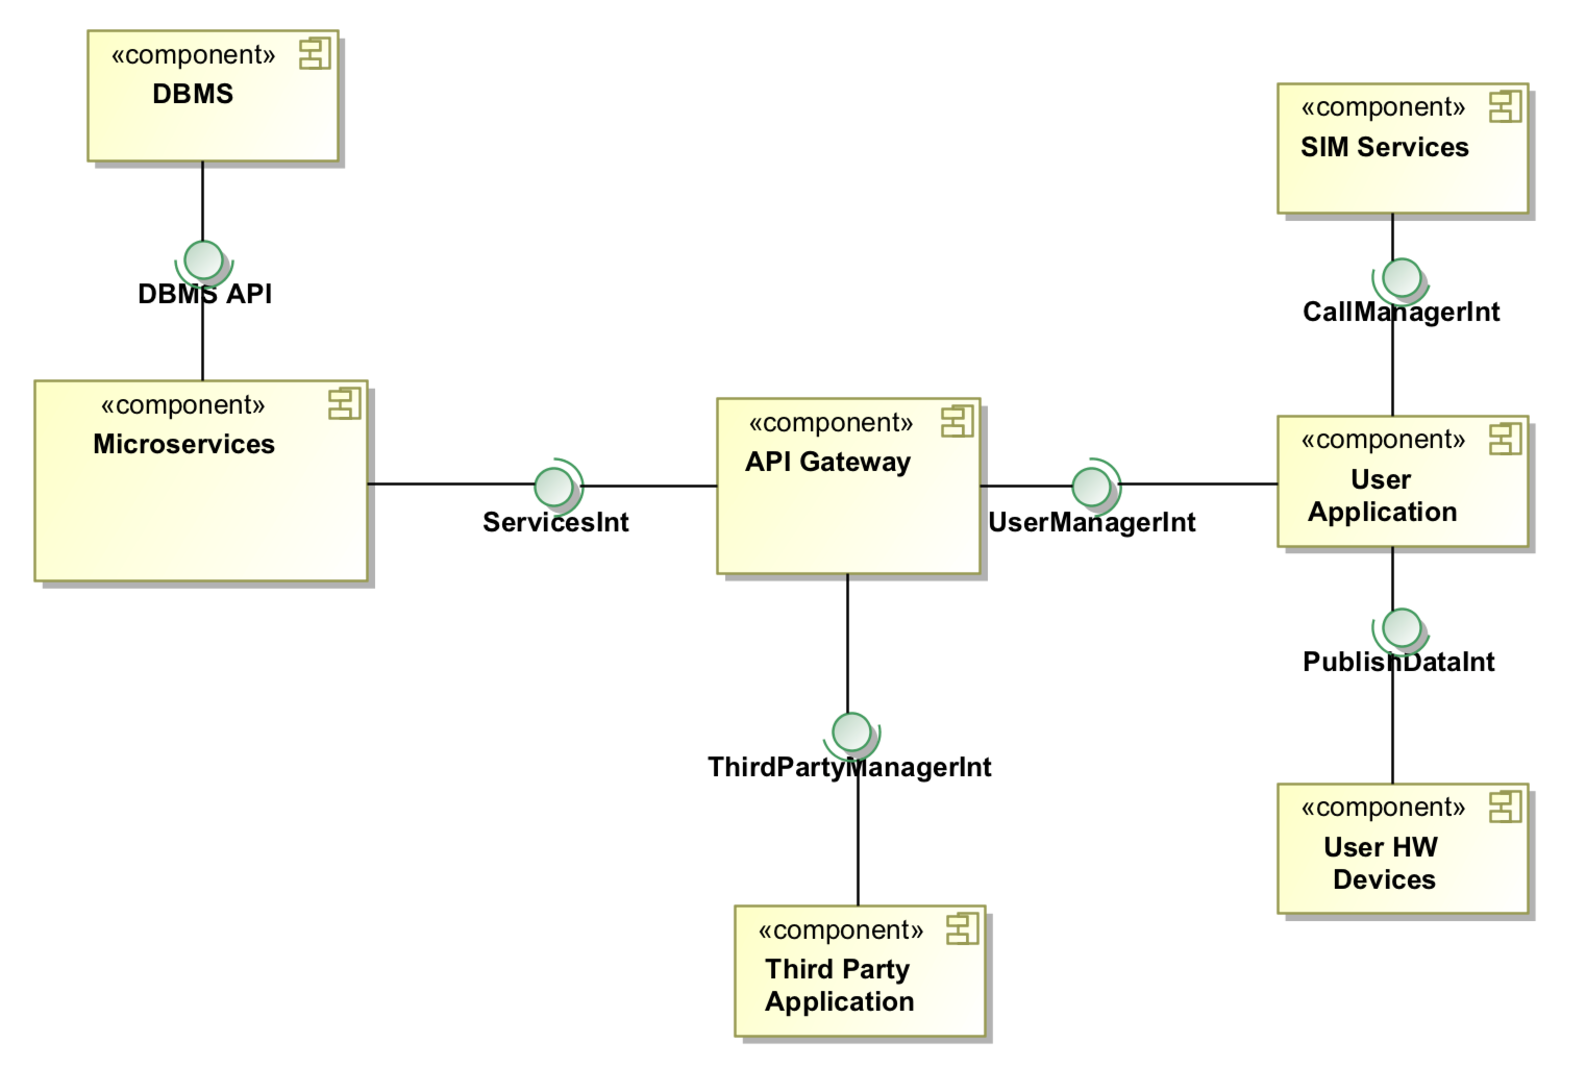
\includegraphics[width=\linewidth]{Images/highlevelcd.pdf}
\caption{ High-level component diagram }
\label{fig:highlevelcomponentdiagram}
\end{figure}

As a reference architecture, the microservices one has been considered: this decision will be later discussed. \\
From the picture, it is evident that the clients can access the services by means of an API gateway, that will provide authentication 
to the users, and forwards the requests to the correct microservices based on the service registry.
Of course, a new service instance needs to register to the service registry in order to be located by the API gateway. \\
Another relevant information is that the project can be ideally split, at a high level, into two applications: one for the users and one for the third parties customers: they both interact with the API gateway, that will guarantee to access all the
microservices that compose the core functionality of the business.
More specifically, the "microservices" block includes Data4Help and Track4Run functions, while the goals
of AutomatedSOS service are reached locally and directly by means of the user application, that, when
needed, will perform a call with the help of the SIM service. 
The user application also needs to communicate with a device that is able to collect data regarding his health: more specifically, this
instrument will send data toward the user application autonomously, without being asked.
Examples of  this machines are smartrings and smartwatches. 
The data regarding the position of the user is, instead, retrieved via GPS's API. \\
Note, also, that the microservices need to keep some data persistent, and, thus access to a DBMS, by means
of its API. 
Moreover, some services need also to communicate and share information: this is achieved via the message queue, that is
charged of receiving and forwarding messages to the interested parts. \\


\subsection{Component view}
In this section, components are expanded and better analyzed. \\
The main analysis regards the microservices block: 
\begin{figure}[H]
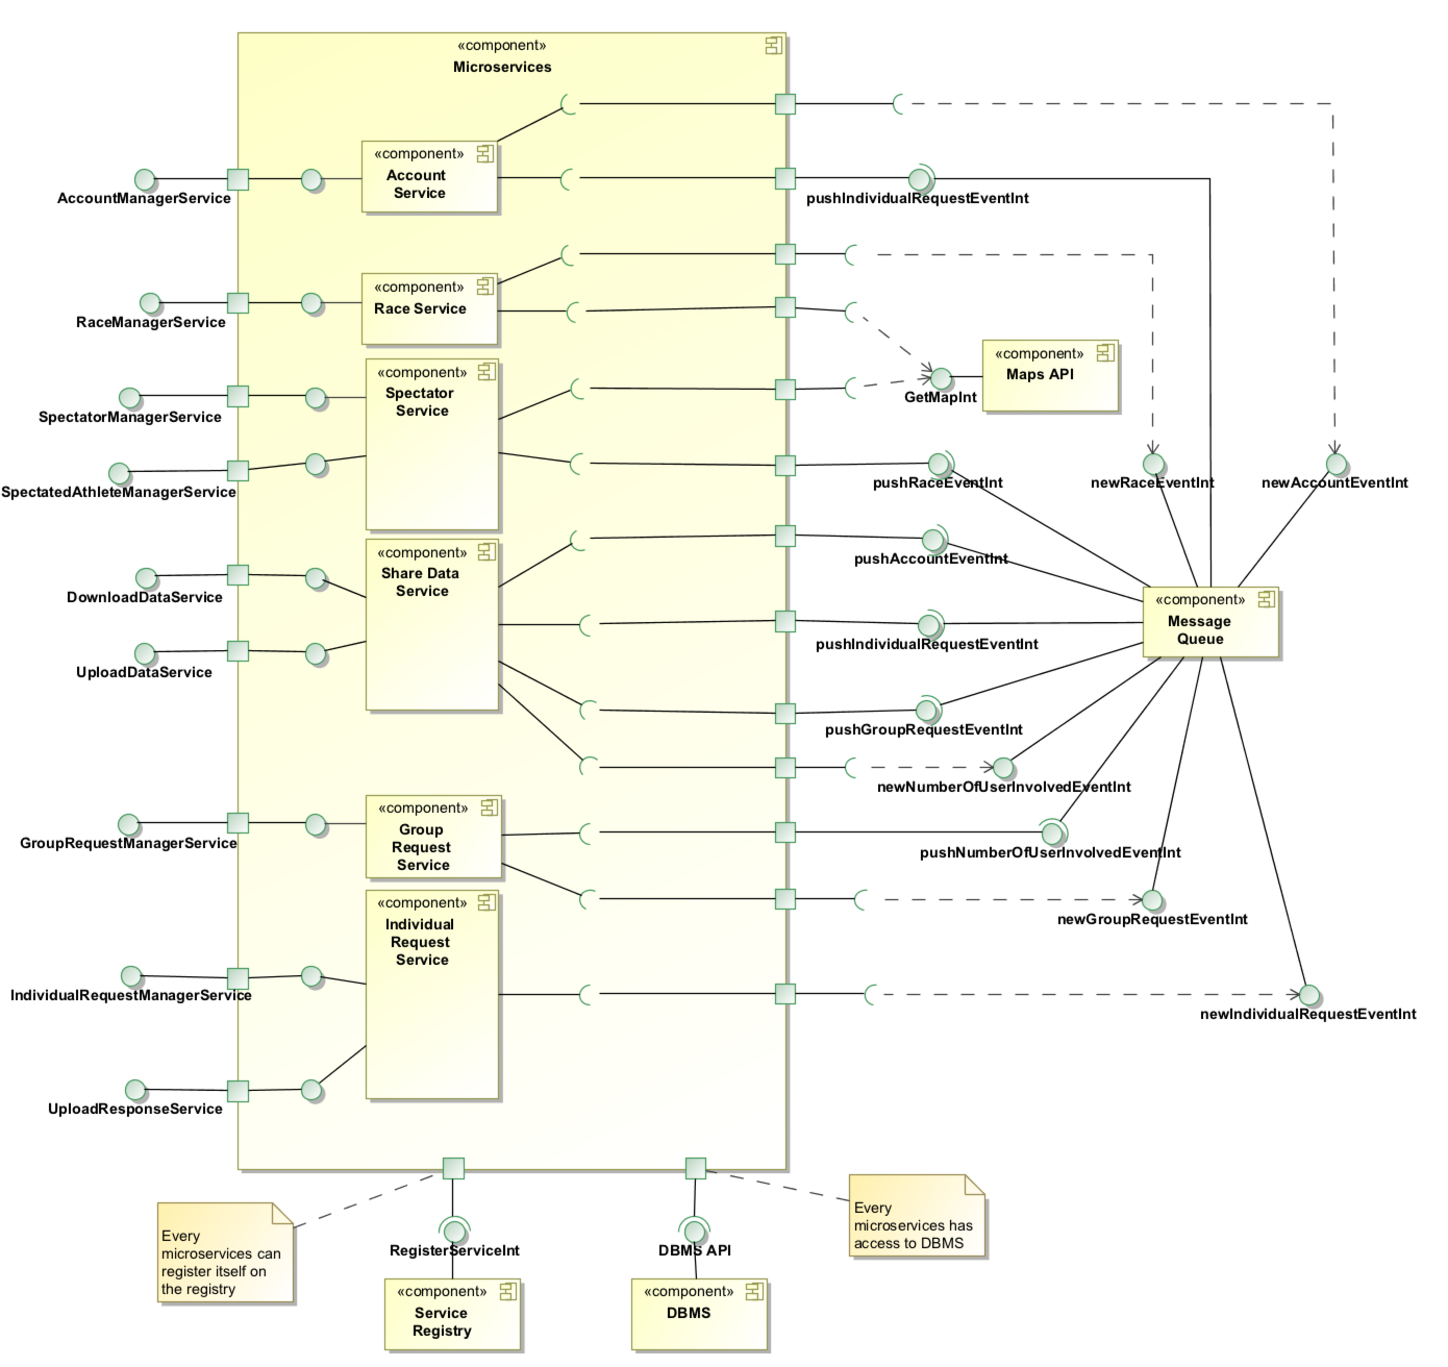
\includegraphics[width=\linewidth]{Images/componentdiagram.pdf}
\caption{ Component diagram }
\label{fig:componentdiagram}
\end{figure}
Various service components are present, and they all expose at least an interface that is accessed by the
clients via the joint combination of API gateway and router.
It follows a brief description of the various services, and a better specification of the interfaces they provide to users and third party customers:
\begin{itemize}
\item The account service provides all the functions related to user sessions, such as login and logout,
and also the registration of clients 
\item The race service makes possible for an athlete to enroll in a run; for a third party customer to set
up one, and also close it; and it also enables the possibility of retrieving the available races and their
status (e.g. in course, terminated). Therefore, it manages the "more static" part
of a race
\item The spectator service regards the dynamic part of a race, such as the fact that a user can spectate
athletes who are running (therefore they can retrieve their positions and the leaderboard). This
service is also in charge of receiving position data of the participants
\item Share data service is responsible for the monitoring the user health statuses and positions: here a
user will upload his data. Furthermore, third party customer will access the data that they have
previously requested, by means of "AccessDataService" interface
\item The group request service provides to the third parties the possibility of uploading group requests and see their status 
\item The individual request service enables third party customer to upload individual request and monitor their status, and allows a user to
check if there are some requests for him, and, eventually, upload responses 
\end{itemize}

Microservices have their own data and, therefore, access DBMS's API, while Maps's API are necessary 
only for race and spectator service, in order to manage and double check position data and feasible paths. \\
The diagram also shows the main communications that take place between components. 
The following message exchange is needed to completely and correctly exploit the project functions. 
\begin{itemize}
\item 
When a third party is accessing individual data through the data share service, it
needs to know if a request associated with those data was sent and accepted. 
Indeed, the request acceptance and its data, are managed in the following way: when an individual request has been accepted, a message is sent through the message queue with the help of an interface, IndividualRequestEventPublisher. Then, this message reaches the share data service thanks to the interface provided by it (i.e. IndividualRequestEventListener). \\
Moreover, to guarantee that individual requests must be performed on registered users, a match with the account service 
is necessary. When a new user registers, the account service will send the data about the user through the message queue to reach 
all the services which need it. One of these services is the Individual Request Service which needs the user to check if an individual 
request is coherent with the system (UserEventListener and UserEventPublisher are the interfaces that accomplish this task). 
\item 
A slightly different reasoning holds for the management of the group requests. In this case, the exchange is bidirectional. 
In particular, when a new group request is performed, the share data service will be notified by the message queue via the
GroupRequestEventListener, and it will be sent to the message queue by GroupRequestEventPublisher. \\
When the share data service receives this event, it will query its data in order to retrieve information regarding the number of users
involved: of course, this information needs to be sent back to the group request service, that will accept or refuse the request
(DataEventListener and DataEventPublisher are the interfaces that accomplish this task). 
Of course, the acceptance of the request may trigger again the new group request event. 
However, this will be later exposed and commented in the run time view. \\
Moreover, to guarantee that the filters on the aggregated request are applied correctly (e.g. data on the users whose age is greater then 40)
a match with the account service is needed. 
Indeed, when a user registers to the service, the account service will sends user information to the message queue with UserEventPublisher. 
The information will be forwarded to the share data service with UserEventListener.
\item
Another important message exchange is between spectator and race services: in particular, data that the spectator service is receiving must
be matched with an active run, and thus it needs to know the status of the run: the changes will be communicated by 
RaceEventListener and RaceEventPublisher.
\end{itemize}

\subsection{Deployment view}
\par
Regarding the deployment, there are many quality to take into consideration. One of these is the scalability property: at the beginning 
TrackMe might only have few users, but once the usage is increasing more and more, the system must continue to work even if the 
requests from the users are huge. To achieve this quality of service, TrackMe needs the help of cloud database providers. These ones 
are specialized in the management of big database; and in this case the Share Data Service require a huge database in order to store 
all the data collected from the users. 
\par
On the other side, services such as Account Service, Individual Request Service and Group Request Service do not require so much 
power. Therefore, a good solution is the virtualization; in such a way each microservices has its own application server, while 
the database server can be shared among these services.. Instead, Spectator Service require to save a good amount of data and 
the access might be frequent due to the requirement regarding the possibility to see all the positions of the runners during a race. 
Consequently, Spectator Service has its own database 
server machine.
\par
To access these microservices one needs to use the mobile application which has to be installed either on an Android device or on a iOS 
device; Firewalls are used to separate the client domain and the server domain, and also used to filter packets which can be malevolent.
\begin{figure}[H]
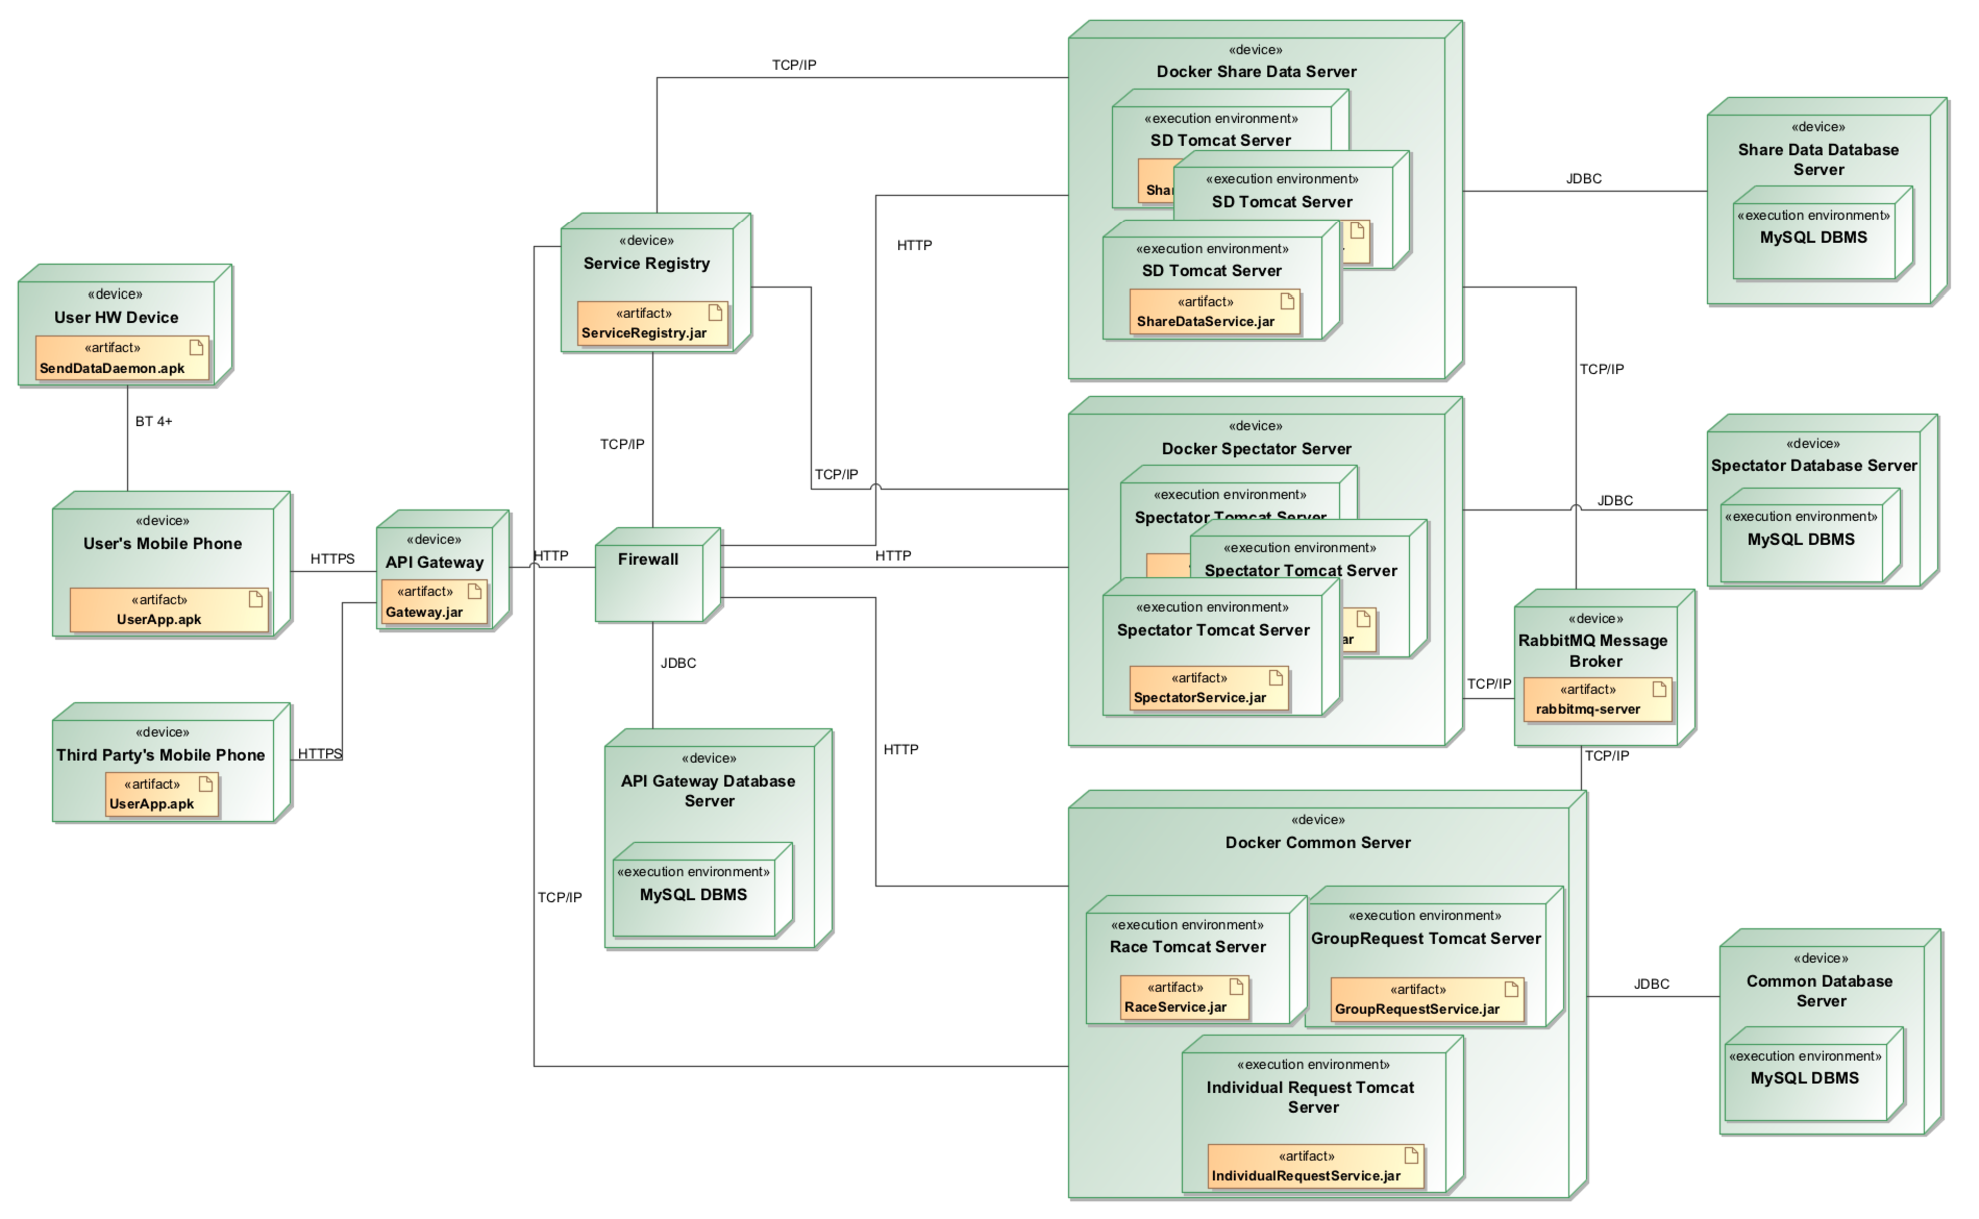
\includegraphics[width=\linewidth]{Images/deploymentdiagram.pdf}
\caption{ Deployment diagram with Archimate }
\label{fig:deployment}
\end{figure}
The deployment diagram represents the system to-be which is based on the microservices "reference architecture". Even if 
microservices offer the possibility to implement different services with different programming language or framework, what is simpler 
is to keep using the same environment. In this case, Glassfish application server and Oracle DBMS are strongly used. In conclusion, 
the system can be also seen as clients and many servers with 4 tier:
\begin{itemize}
\item Tier 1: Client side, which is the presentation
\item Tier 2: API Gateway, which redirects all the requests from the client to the respective application server
\item Tier 3: Application servers, which contains the logic business of the system
\item Tier 4: Database servers, in which it contains all the data
\end{itemize}
\subsection{Runtime view}

\subsection{Component interfaces}
Here follows the interfaces of the various components that are available. 
Note that interfaces of external components (e.g. DBMS's API, CallManagerInt, GPSInt, MapsAPI) are not present. 

\begin{figure}[H]
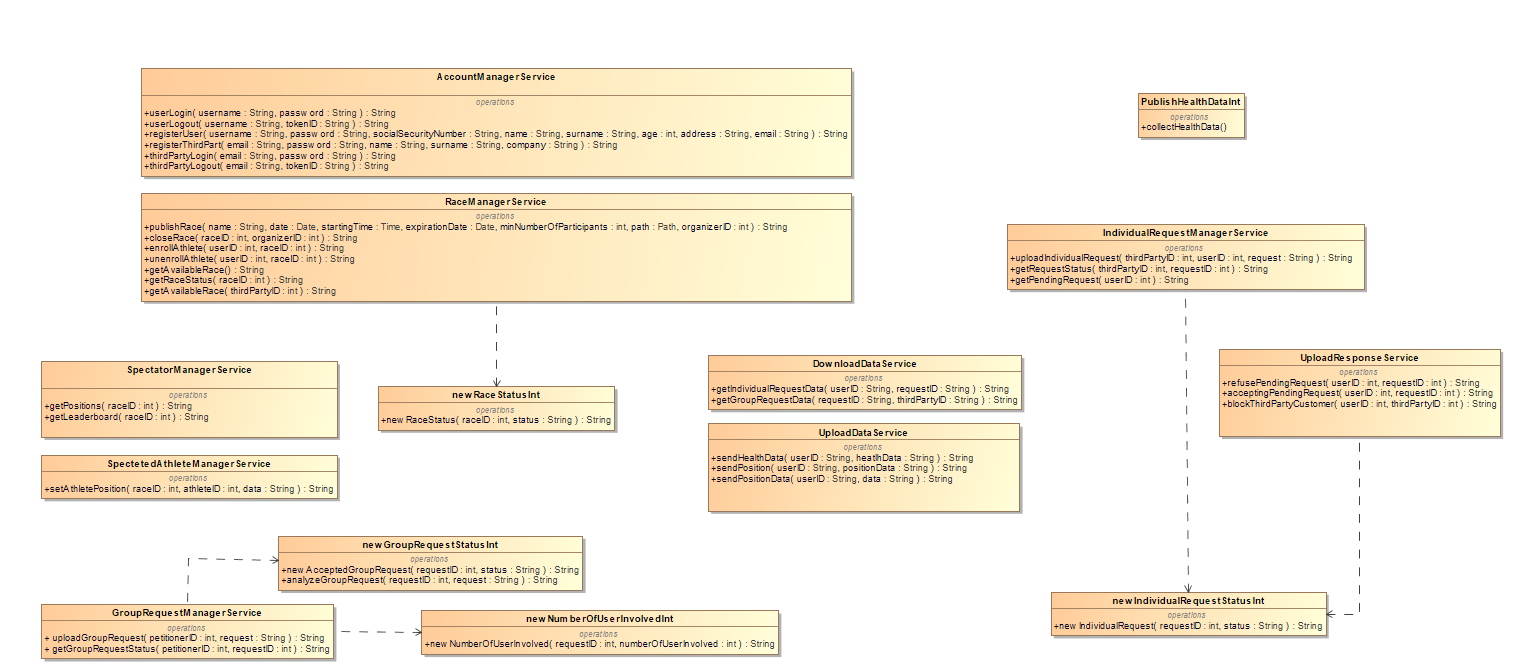
\includegraphics[width=\linewidth]{Images/componentinterfaces.png}
\caption{ Component interfaces }
\label{fig:componentinterface}
\end{figure}

In order to simplify the diagram, the API gateway has been excluded, but what it exposes is just the following: it provides a link for each
interface that is external w.r.t. the microservices block in figure \ref{fig:componentdiagram}. However, there is a little modification in the
parameters requested: indeed, the id of the client that is requesting the service (e.g. userID, thirdPartyID, athleteID) is substituted with
tokenID, in order to manage the authentication. This holds, clearly, with the exception of the registration and login feature, since a token 
is not available at this early stage of the user session. \\ 
A same reasoning is applied for what concerns the router: it just forwards the "translated" requests.
\subsection{Selected architectural styles and patterns}
In this section, all the adopted architectural styles and patterns are explained sufficiently to define why the specific style or pattern is chosen.

\subsubsection{Microservices}
The selected architectural style, as already mentioned, is the microservices architecture. This choice is
supported by multiple reasons. In particular, a strong motivation in the decision process is the
conjunction of the following two facts:
\begin{enumerate}
\item Data4Help and Track4Run are features that provides totally different and independent functions.
Track4Run can, without any problem, even be deployed in a different moment
\item Scalability is one of the main QoS that the system requires. Indeed, the application is expected to
be used by many people in the future, and therefore, designing the architecture making scaling fast is
really important
\end{enumerate}
It is important to note that it could happen that one of the two functions needs to scale, while
the other does not. 
More specifically, this reasoning also applies to some pieces of functionality that
are internal to both Data4Help and Track4Run. 
For instance, it is reasonable to assume that the functions of data collection from users (positions and
health statuses) will be much more used and will generate much more network traffic, compared to the one
that regards the requests. 
In order to clarify this, all the active users will periodically send data at each moment of the day,
while third party customers that are performing requests do not keep forwarding request to the user: it is
something that happens more rarely. 
The same holds, for example, when considering the set up of run events from the organizer, and the fact
that spectators will monitor in real time positions of athletes during a race. \\ 
Therefore, the combination of these things, suggests that the scaling should be independent w.r.t. the
function considered. \\
Furthermore, the microservices architecture makes it easier to implement failure isolation: it is not
desirable that a failure in Track4Run leads in a failure in also Data4Help. 
Moreover, failing in managing the request should not prevent the data collection: as one can see the
reason also applies to the various business capabilities that are bounded in the single Data4Help, or
Track4Run, feature.  
Due to this, the overall availability is improved. 

\subsubsection{Eventually consistency and compensation}
Before going to analyze all the patterns adopted for the microservices architecture, one must define the most important thing in a microservices architecture: how to achieve consistency of data. For instance, solutions for this issue are:
\begin{itemize}
\item Avoiding transactions across microservices: usually if a microservices architecture needs to have distributed transactions 
it means that there are redundant data. But if this is avoided, the lack of redundant data means that everytime a microservice needs 
to ask data from another microservice, a request is sent and if the other microservice is under high load, it will not be able to 
process it fast.
\item Two-Phase commit protocol (2PC): The distributed transaction of 2PC consists on two steps: Prepare phase (lock-phase) 
and Commit-rollback phase (unlock-phase). The problem with this protocol is that it is too slow compared to the time for an 
operation of a single microservice.
\item Eventual consistency and compensation: it is a model different from ACID transactions, but it is a mechanism to 
achieve consistency eventually at some point in the future. This might not achieve the same thing as 2PC but it is faster and if 
the architecture does not need the strict properties of ACID, then it is better. Otherwise, it could be very difficult to implement it.
\end{itemize}
Out of the three solutions, 2PC is not an option since the messages are synchronous, which means too slow. Therefore, Eventual consistency and compensation is the one adopted by this project due to the fact that the system will scale a lot and there is no problem if consistency is achieved in the future.


\subsubsection{Design patterns}
Now, some patterns adopted related to the microservices architecture are exposed:
\begin{itemize}
\item API gateway: this is a component already introduced in the high level component diagram and it
satisfies and deals with the following problem: how do clients of the application access to the individual
services? The API gateway is a single entry point for all clients and it can expose different API for
each client: this suits well for the TrackMe project. This should be implemented with an event-driven
reactive approach in order to scale if it is necessary to manage big loads of data \\
\item The access token pattern is very useful, since the application is composed of various services and
an important issue is how to communicate the identity of the petitioner to the service that handles the
request. 
The pattern suggests to implement the API gateway in such
a way that it authenticates requests and passes an access token that securely identifies the client (a
service may later include the access token in requests that it makes to other services)
\item Database per service pattern: all the services need to persist data in some kind of databases and
the solution is to keep each microservice's data private to that service and accessible only via its API.
So a database can't be accessed directly by another service. In particular the pattern of schema-per
service is always guaranteed, while a database-server-per-service is allocated to the services that are
though to be the one with the highest throughput (i.e. spectator service and share data service)
\item The messages and the communications between services, that were already introduced in the component diagram, are implement by means of
asynchronous messages, since a chain of synchronous calls could lead to slowdown the entire architecture. Note, that this leads to the
replication of some data, however, performance is considered more important than cost in this case. A way to achieve a better communications between services is to use something similar to the API gateway: a message queue architecture which requires also an additional service called message broker that is responsible for gathering, routing and distributing messages from services to other services (something similar to a mail service)
\item 
As shown, services need to call one another, but a microservices-based application typically runs in a virtualized 
environment where the number of instances of a service and their locations changes dynamically. 
The solution is to use a router that runs at a well known location. 
The router will query a service registry, which may be built into the
router, and forwards the requests to an available service instance.
Of course, when a new instance is created, it has to perform registration to the service registry. \\
The API gateway will send translated requests to the router, that will load balance them onto the active instances.
This pattern gives great benefits: indeed, the clients do not deal with the discovery of the service, but it comes with the drawback of
an additional component that need to be installed and configured, and, if needed, replicated, in order to scale
\item Microservices expose REST API that will be provided only by HTTPS endpoints. This will ensure
all the benefits of REST API, such the fact that services are stateless, with the security of an high-level encryption protocol. Other
benefits of the REST API which are relevant to the requirements of the project are: separation of concerns between client and server, reliability and scalability.
\item Saga pattern: this design pattern is, practically, a way to achieve the solution of Eventual consistency and compensation described before. It solves the trouble of distributed transactions without using 2PC by using a sequence of local transactions where each transaction updates data within a single service. Even though 2PC guarantees ACID properties, it is better Saga pattern that achieves only different properties, called BASE: Basic Availability Soft-state Eventually consistent.  But with Saga, there are two main different ways to implement a saga transaction:
\begin{itemize}
\item Events/Choreography: each service subscribes and publishes to other service's events
\item Command/Orchestration: there is a central coordinator service which is responsible about decision making and sequencing business logic 
\end{itemize}
In the project it is implemented the version of event transaction. Other than this implementation, Saga pattern defines also 
the compensation action: an action to restore the original states if there are failures during a distributed transaction (e.g. in 
the individual request service, if a third party sends a request regarding a non-existing social security number, then when 
account service is triggered, it will send a compensation action to the individual request by saying that the request must be canceled).

\end{itemize}
\subsection{Other design decisions}
\subsubsection{Frameworks}
The chosen and described architectural style, leads to some choices in the framework that will be used for the development and the deployment. 
In particular, to implement a microservices architecture, a microservices chassis framework is needed, in order to have the best support 
in the developing phase. 
An option here is to adopt both Spring Boot (for what concerns the microservices) and Spring Cloud (that facilitates the set up of distributed
system software). They are widely adopted and greatly supported by the community; also many guides and articles are available on the internet. \\

\subsubsection{Asynchronous messages}
RabbitMQ, that is a message broker server, is used to implement the exchange of messages among services. This choice is motivated 
by the following facts: it enhances delivery and order guarantee, redundancy, decoupling and scalability. 
Finally, it is well supported in Spring boot. 

\subsubsection{Data transfer encryption}
Another important issue is regarding the communication between the user hardware device and the user application. This is encrypted with
AES-128. \\
The communication happens by means of bluetooth: the version 4.0 + LE, that is available from 2010, provides some nice features for the
project, because it grants enough bandwidth (1Mbps when the low energy mode is enabled) for transmitting the data, and it is also a low
energy consumer. Furthermore, there is no need of internet connection (with the limits of the network coverage): the devices just need to be
close, but this is a totally rational assumption, given the context of the application. 
Note that this version ensures a good compatibility with a large set of devices. 

\subsubsection{Android application} 	 
The user application will be developed for the Android operative system, at least in a first moment. This is due to the criticality of the
automatedSOS service. Assuming that the application will be deployed with Italy as the first market target, this choice covers the biggest
part of the market.

\subsubsection{JSON}
REST API will be implemented using JSON as a protocol for exchanging data. \\
Compared to XML, it is less verbose and JSON packets require less size. Furthermore, it is well supported
by Spring Boot. 

\subsubsection{Group Request Filtering}
Up until now, group requests were more or less abstract: there was no definition of what group requests could possibly get from 
data. Therefore, here it is defined what group requests return. The only outcomes they give are  aggregated data, i.e. count 
of tuples, sum of values, average of values or other aggregate operator available (e.g. in SQL). Another thing to clarify is that 
the tuples of the result from a group request have to satisfy a certain constraint requested by the petitioner. Consequently, 
the following filters are the ones available:
\begin{itemize}
\item Filtering by birth city
\item Filtering by birth nation
\item Filtering by birth year
\item Filtering by the GPS position data
\item Filtering by the health statuses
\item Filtering by date and time
\end{itemize}
Since this type of service is very difficult to implement for the user (user-friendly difficult), each filter is applied to decrease the number of users and every query is applied only to users that have at least one position data and one health data. Basically there is no group-by statement in the query.







\newpage

\section{User interface design}


\newpage

\section{Requirements traceability}
Below are listed the design components to which Data4Help requirements and goals are mapped: 
\begin{itemize}
\item[{[G1]}] Allow a user to access its own data. Requirements([R10])
	\begin{enumerate}
	\item Account service.
	\item Share data service.
	\end{enumerate}
\item[{[G2]}] Allow a user to contribute to data sharing by providing information about his location and health status. Requirements([R11])
	\begin{enumerate}
	\item Share data service.
	\end{enumerate}
\item[{[G3 \& G4]}] Once the health parameters of a user have been observed below the threshold for the first time after one hour, an ambulance is sent to the user location. 
The time experienced between the moment in which the health parameters of a subscribed user are observed below the threshold and the time in which the emergency point is contacted is equal or less than 5 seconds. Requirements([R12]-[R13]-[R14]-[R14]-[R15]-[R16]-[R17])
	\begin{enumerate}
	\item Share data service.
	\item SIM services.
	\end{enumerate}
\item[{[G5]}] Allow a user to participate in a run managed by third parties, as an athlete, if all starting conditions are satisfied. Requirements([R18]-[R19]-[R20]-[R21]-[R22])
	\begin{enumerate}
	\item Race service.
	\end{enumerate}
\item[{[G6]}] Allow spectators (i.e. user) to see on real-time the "correct" positions of all athletes taking part in a run, with at most 15 meters of radius error.
Requirements([R23]-[R24])
	\begin{enumerate}
	\item  Spectator service.
	\end{enumerate}
\item[{[G7]}] The maximum time to accept an individual request from any third party is 30 days; after that, the request will expire. Requirements([R25])
	\begin{enumerate}
	\item Individual request service.
	\item Group request service.
	\end{enumerate}
\item[{[G8 \& G9]}] Allow a user to accept or refuse a request from third parties. Allow a user to block requests made by a specific third party. Requirements([R26]-[R27]-[R28]-[R29])
	\begin{enumerate}
	\item Individual request service.
	\end{enumerate}
\item[{[G10]}] Allow spectators and runners to see the leader board, when a run is completed. Requirements([R30]-[R31]-[R32])
	\begin{enumerate}
	\item Spectator service.
	\end{enumerate}
\item[{[G11]}] Allow organizers (i.e. third parties) to set up a run, by defining its name, its path, date, start time, expiration date, and the minimum number of participants. Requirements([R33]-[R34])
	\begin{enumerate}
	\item Race service.
	\end{enumerate}
\item[{[G12]}] Allow a third party to access data specified in a request if the user accepts the request or if he accepted one or more requests from the same third party that provided access to the same data. Requirements([R35]-[R36]-[R37]-[R38])
	\begin{enumerate}
	\item Individual request service.
	\end{enumerate}
\item[{[G13]}] Allow a third party to access statistical and anonymized data if and only if the number of individual involved is greater than 1000. This is satisfied as soon as the request is approved. Requirements([R39]-[R40]-[R41]-[R42])
	\begin{enumerate}
	\item Group request service.
	\end{enumerate}
\item[{[G14]}] Allow a third party to subscribe to non-existing data. They will have access to them, as soon as the data is generated. Requirements([R43]-[R44])
	\begin{enumerate}
	\item Individual request service.
	\item Group request service.
	\end{enumerate}
\end{itemize}

\newpage

\section{Implementation, integration and test plan}

\newpage

\section{Effort Spent}

\subsection{Riccardo Poiani}

\begin{table}[H]
\begin{tabularx}{\textwidth}{|l|X|c|}
\hline
\rowcolor[HTML]{C0C0C0} 
Date & Task & Hours\\ \hline
15/10 & Goal definitions & 2.5\\ \hline
17/10 & Document structure, goal definition, class diagram & 2.5\\ \hline
18/10 & state diagram, class diagram, purpose, hypothesis & 1.5\\ \hline
19/10 & Scope, purpose and state diagram & 2\\ \hline
22/10 & Product functions & 2\\ \hline
23/10 & Scenarios & 2\\ \hline
24/10 & Scenarios & 1\\ \hline
25/10 & Refactor all document (revising) & 1\\ \hline
26/10 & Refactor all document (revising) & 4\\ \hline
27/10 & Add design standards, performance, availability, reliability, security; Add use case diagram and sequence diagram & 5\\ \hline
27/10 & Alloy & 2\\ \hline
28/10 & Alloy; world and shared phenomena; use case; whole document revision; sequence diagram & 7.5  \\ \hline
29/10 & Alloy; sequence diagram; fix requirement& 3 \\ \hline
01/11 & Revise document & 4 \\ \hline 
\rowcolor[HTML]{C0C0C0} 
& Overall & 40 \\ \hline
\end{tabularx}
\end{table}

\subsection{Mattia Tibaldi}

\begin{table}[H]
\begin{tabularx}{\textwidth}{|l|X|c|}
\hline
\rowcolor[HTML]{C0C0C0} 
Date & Task & Hours\\ \hline
15/10 & Goal definitions & 1.5\\ \hline
17/10 & Introduction & 2\\ \hline
18/10 & Scope and purpose & 4\\ \hline
19/10 & State diagram & 1\\ \hline
22/10 & Hardware interfaces & 2\\ \hline 
23/10 & Software interfaces & 3.5\\ \hline
24/10 & User interfaces & 3\\ \hline
25/10 & User interfaces and communication interfaces & 4\\ \hline 
27/10 & Revise document and use case & 3.5\\ \hline
28/10 & Alloy & 4.5\\ \hline
29/10 & Alloy and refactor document & 4\\ \hline
01/11 & Revise document & 4 \\ \hline 
\rowcolor[HTML]{C0C0C0} 
& Overall & 36\\ \hline
\end{tabularx}
\end{table}

\subsection{Tang-Tang Zhou}

\begin{table}[H]
\begin{tabularx}{\textwidth}{|l|X|c|}
\hline
\rowcolor[HTML]{C0C0C0} 
Date & Task & Hours\\ \hline
15/10 & Goal definitions & 2.5\\ \hline
17/10 & Document structure, goal definition, class diagram & 2.5\\ \hline
18/10 & state diagram, class diagram, purpose, hypothesis & 1.5\\ \hline
20/10 & Product Perspective, race diagram, request diagram and Alloy & 4\\ \hline
21/10 & Alloy & 1.5 \\ \hline
22/10 & Fix goals, purpose and perspective & 2\\ \hline
23/10 & Domain asssumptions and requirements & 2\\ \hline
24/10 & Requirements, goals, assumptions & 2\\ \hline
25/10 & Refactor all document (revising) & 2\\ \hline
26/10 & Refactor all document (revising) & 3\\ \hline
27/10 & Fix requirements, add alloy, add use case and sequence diagram & 5\\ \hline
27/10 & Add mantainability, portability, definitions, structure and references & 2\\ \hline
28/10 & Revise document, fix diagrams, add sequence diagram to document, add effort spent & 5\\ \hline
29/10 & Fix diagrams, Add alloy worlds, fix requirements & 2 \\ \hline
31/10 & sequence diagram & 1 \\ \hline
01/11 & Revise document & 3 \\ \hline 
\rowcolor[HTML]{C0C0C0} 
& Overall & 41\\ \hline
\end{tabularx}
\end{table}

\newpage

\end{document}


\section{Structure of the source code}

\subsection{Microservices}
Here the code regarding the microservices architecture is explained. \\
The source code that meets the requirements mentioned above has been organized in the following way: for each microservices a project
has been set up. 
Indeed, when dealing with this type of architecture, one should think of a microservice
as a project that should be as much independent as possible from the others: this is the reason that stands behind the choice that has been
made. 
Of course, in this way, it is possible to easily generate the single jars that will be deployed, when necessary, with, as mentioned
in the design document, dockers. Therefore, the following projects are present: API gateway, service registry, group individual request
service, individual request service and share data service. 
As one may notice, the one containing the set up of the API gateway also accesses all the information related with the accounts, and, therefore, authentication and authorization functions are coded here.
In the following sections the structure of the single projects are analyzed. 

\subsubsection{API Gateway}
In the figure ~\ref{fig:pkgapigateway}, it is shown the root of the project structure. An analysis 
of the various elements follows below the figure. 
\begin{figure}[H]
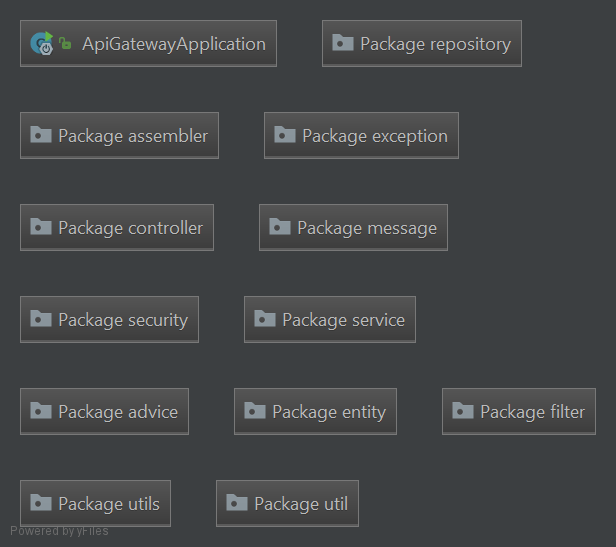
\includegraphics[width=\linewidth]{images/PackageApigateway.png}
\caption{ API gateway }
\label{fig:pkgapigateway}
\end{figure}

\begin{itemize}
\item Package repository: contains the JPA repository for accessing the persistent data necessary to this
service. 
In particular information regarding the accounts of users and third party customers are present. For what concerns the third party customers,
since they can register both as private and as related with a company the following repositories are present: company details, private
details, third party customers and users. An additional repository is present, and it accesses information regarding the API. Indeed, all
the accessible APIs that are available are stored in a database, in order to provide access control. For better specifying this choice, 
one may consider the fact that it is not necessary to search on the service registry non-existing API or to forward requests that can
be already classified as rejected (e.g. user A that is trying to access an API available only for third party customers)
\item Package assembler: this class contains components useful to build HATEOAS resources of entities that are returned to clients, adding
hypermedia contents
\item Package exception: this contains the custom exceptions defined during the development
\item Package controller: contains the controller that defines the APIs that regards the management of the users and third party customer
accounts. From here, it is possible to access the business functions that regards the account (e.g. login, logout, registration). Inside here,
controller are split into secure and public controllers: the public one are accessible to everyone, while for accessing the secured ones,
it is necessary to perform the log in
\item Package message: it provides the functions of communicating with other microservices, by means of RabbitMQ. In particular, three
subpackages are present here. The package publisher contains classes that helps in publishing the events of creation of new accounts to other 
services. The package protocol defines a way of communicating the interested pieces of information, and, finally the configuration
package specifies the configuration settings needed to convert object from JSON (and viceversa) during the propagation of data and also RabbitMQ exchanges and queues\cite{rabbit-concepts} .
\item Package security: contains the main features that have been introduced above regarding the security 
\item Package service: contains the services that implements the business functions of the account service, with all the APIs that it exposes.
The interfaces present here map the component interfaces of the account service
\item Package advice: this encompasses the handling of server side exceptions in order to show to clients useful messages without exposing
the structure of the project and low level errors
\item Package entity: here classes that are mapped to the databases are present   
\item Package filter: it includes filters that the API gateway applies during the management of "external" requests (i.e. requests that
need to be processed by other services). In particular, it is further subdivided into three packages: pre, route and post. In this case, the
pre filter that is present perform access control on the external API that is being requested, the route filter is a translation filter
that adds header in order to identify the clients in the other microservices, and the post filter fixes the hypermedia content that is sent
as a response to the original request
\item Package util: various utility needed in the development
\end{itemize}

The routes to the other microservices available are present in the application.properties file.
Here it follows a list of the API available:
\begin{itemize}

\item /public/users/authorize \\
This requires two request parameters, that are username and password. This API is necessary to login the users.
The method is POST.

\item /public/users/\{ssn\} \\
This is the entry point for registering a new user. Here, ssn is a path variable that specifies the social security number
of the user that will register. A request body that specifies the necessary fields of the JSON are specified in the user entity. \\
Here it is reminded that one should check the needed fields paying attention also to the defined JSON views defined. \\
This holds also for the other methods in which a request body is needed. \\
The method is POST.


\item /public/thirdparties/authorize \\
This requires two parameters, that are email and password. This API is necessary to login the third party customers. 
The method is POST.

\item /public/thirdparties/companies is necessary to register a third party customer that is related with a company. \\
A request body is needed to specify all the information related to that customer. The method is POST.

\item /public/thirdparties/privates is necessary to register a third party customer that is not related with a company.
A request body is needed to specify all the information related to that customer. The method is POST.

\item /users/info returns the information of the user that is accessing that API. The method is GET.

\item /users/logout performs the logout of the user from the system. The method is POST.

\item /thirdparties/info returns the information of the third party customer that is accessing the method. The method is GET.

\item /thirdparties/logout performs the logout of the third party customer from the system. The method is POST.

\end{itemize}


\subsubsection{Service registry}
The project of the service registry is almost empty, no package is present, but just an application class annotated with 
@EnableEurekaServer. The configuration of the service registry is set in the application.properties file.

\subsubsection{Group request service}
In the next figure, the package diagram of the group request project is shown ~\ref{fig:pkggrouprequest}. \\
The same comments hold here except for the fact that the business function mapped in the component interfaces are the one regarding
the group request service. 

\begin{figure}[H]
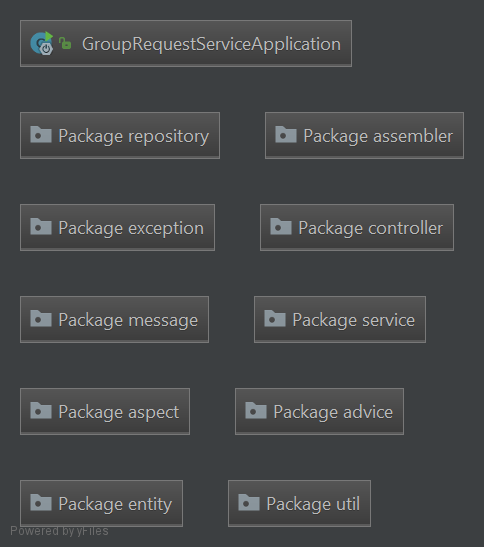
\includegraphics[width=\linewidth]{images/PackageGrouprequestservice.png}
\caption{ Group request service }
\label{fig:pkggrouprequest}
\end{figure}

Here it follows a list of the API available:
\begin{itemize}

\item /grouprequestservice/grouprequests/id/\{id\} \\
It retrieves the information related with the group request specified by the id in the
path variable. 
The method is GET.

\item /grouprequestservice/grouprequests/thirdparties \\
It collects all the group requests related with the third party that is accessing the method. 
The method is GET.

\item /grouprequestservice/grouprequests/thirdparties \\
This adds a new group requests. It requires a request body that contains all the details of the group
request that will be added.
The method is POST.

\end{itemize}

The prefix /grouprequestservice is necessary in order to access the APIs from the API gateway. 
Note, that by inspecting the controller, the prefix won't be shown at all: this is because the API gateway does this translation 
and mapping autonomously. Instead, one may notice some request headers: they are added at runtime by the gateway, and so the client
does not have to specify them, and, if it does, they will be overwritten. \\
This comment holds, as well, for all the other microservices.


\subsubsection{Individual request service}
Here it follows the package diagram of the individual request service project ~\ref{fig:pkgindividualrequest}. 
As one may notice, the structure is very similar to the one explained in the api gateway project. 
Of course, here, the controllers provide access to the APIs that regards the individual request service. 
The business functions of this project are present in the  service package, and the interfaces that are present, 
are mapped with the component interfaces of the Design document. \\
Another difference w.r.t. the API gateway that is worth to point out is that here the package message contains also a subpackages that
defines listeners: these are charged of listening to new events that are forwarded from RabbitMQ. 

\begin{figure}[H]
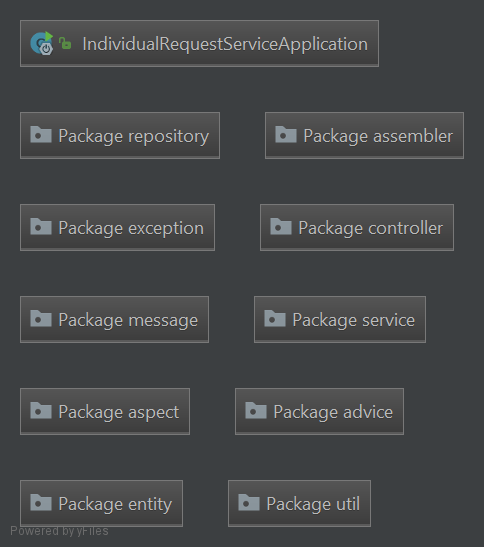
\includegraphics[width=\linewidth]{images/PackageIndividualrequestservice.png}
\caption{ Individual request service }
\label{fig:pkgindividualrequest}
\end{figure}

Here it follows a description of the available API:
\begin{itemize}
\item /individualrequestservice/requests/id/\{id\} \\
This retrieves an individual request identified by means of a certain id. 
The method is GET.

\item /individualrequestservice/requests/users \\ 
This retrieves the pending requests of the user that is accessing the method. 
The method is GET.

\item /individualrequestservice/requests/thirdparties \\ 
This retrieves the requests performed by the third party customer that is accessing the method.
The method is GET.

\item /individualrequestservice/requests/\{ssn\} \\
This adds a new individual request toward the user specified in the path variable.
A request body specifies the information requested to define the individual request.
The method is POST. 

\item /individualrequestservice/responses/requests/\{requestID\} \\
It is used in the case in which the user that is accessing the method
sends a response to the request identified by requestID in the path variable.

\item /individualrequestservice/responses/blockedThirdParty/thirdparties/\{thirdParty\} \\
It is used in the case in which the user that is accessing the method blocks the third party identified by the id specified in the path variable
\end{itemize}

\subsubsection{Share data service}
The structure of the share data service, as shown by the following picture, is also very similar to the previous ones 
~\ref{fig:pkgsharedata}.

\begin{figure}[H]
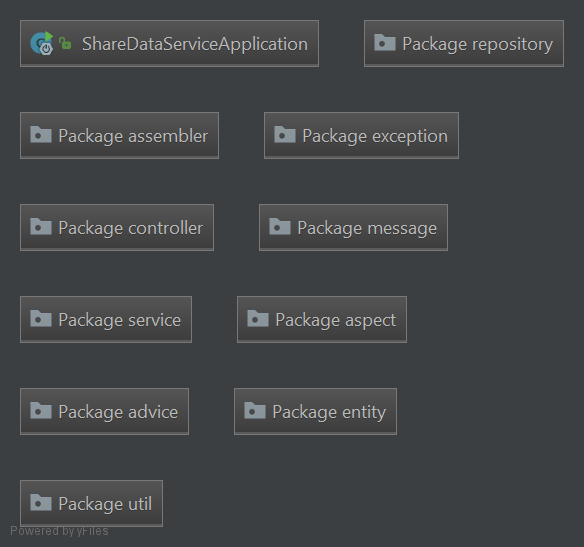
\includegraphics[width=\linewidth]{images/PackageSharedataservice.png}
\caption{ Share data service }
\label{fig:pkgsharedata}
\end{figure}

However, it is important to point out the structure of the code that manages the personalized query specified by the group requests on 
anonymized data. Basically, the custom query is realized with the help of QueryDSL, a sort of unified library to make queries; this choice comes from a limitation of Spring JPA: the impossibility to make union with dynamic queries. Therefore, after researches of other libraries supporting JPA, the best one and mostly supported by the community was QueryDSL which offers a method to makes JPA SQL queries. First of all it is necessary to say that JPA creates connection between objects of classes  and tuples of the DB; this has great advantages when it comes to use only JPA, but mixing it with other methods of retrieving data such as raw SQL queries could introduce some inconsistency. But thanks to JPA SQL queries it was possible to avoid this problem. In conclusion, the custom query is generally something with this simplified template:
\begin{itemize}
\item SELECT AGG\_OP(Column) FROM User JOIN ON Union(HealthData dynamic filtered, PositionData dynamic filtered) WHERE (sameSSN) AND "other filters of User table"
\end{itemize}
  
Here it follows a list of the main API that have been developed in the project, and that are located
within the various microservices.
It is possible to find these mapping in the controller packages. \\
The methods are expressed from a client point of view: for example, takes into consideration the methods that starts with s 

Here it follows a description of the available API

\begin{itemize}
\item /sharedataservice/dataretrieval/individualrequests/\{request\_id\} \\
This method retrieves the data related to the individual request identified by the path variable. The method is GET.

\item /sharedataservice/dataretrieval/grouprequests/\{request\_id\} \\
This method retrieves the data related to the group request identified by the path variable. The method is GET.

\item /sharedataservice/dataretrieval/users \\
This method retrieves the own data of the user. In this case, two request parameters
are necessary in order to specify an interval of time that involves the interested data.
The method is GET.

\item /sharedataservice/datacollection/healthdata \\
This allows the user to send data regarding the health status to the system. The method is POST.
A request body that specifies the data required.

\item /sharedataservice/datacollection/positiondata \\
This allows the user to send data regarding his position data to the system. The method is POST.
A request body that specifies the data required.

\item /sharedataservice/datacollection/clusterdata \\
This allows the user to send cluster of data (both health and position data). The method is POST.
A request body that specifies the data required.

\end{itemize}



\subsection{Mobile code}

\subsubsection{Data4Help}
The source code of the mobile application has been divided in different packages.
The main idea is to build an application where each component represents a microservice's view: 
they are loaded dynamically and they are assembled for drawing the complete user interface. 
This solution, even if it uses a monolithic approach, works well for relative simple mobile applications and it is more easy to implement. 
Of course, in this way, it is possible to easily generate the single APK that will be installed on the mobile device. \\
It follows an analysis that will focus on what is a service component and how it has been implemented in the code. 
In the project, a user interface component is a container, that is represented by an activity class. 
This classes follow the MVP pattern with delegation, thus allowing to have activities less complex and well structured, since the base
structure of an android application with the only uses of simple activities is a bad practice.
The MVP pattern is matched against the baseUtility package and his main components are: contract (basePresenterInterface and
baseViewInterface),
basePresenter, baseActivity and baseDelegate. \\
The fragment that truly represents the microservice's view are loaded into the activities. 

\begin{figure}[H]
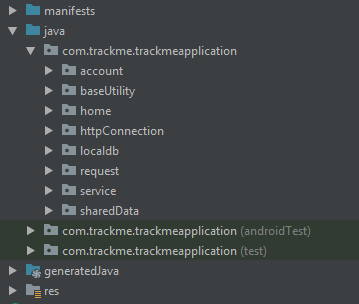
\includegraphics[width=\linewidth]{images/ProjectStructure.png}
\caption{ Code structure}
\label{fig:pkgsharedata}
\end{figure}

In the following paragraph the structure of each package is analyzed.

\paragraph{Account}
In the next figure, it is shown the account package structure and, after that, comes an explanation of the single parts.
  
\begin{figure}[H]
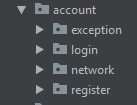
\includegraphics[width=0.6\linewidth ]{images/PackageAccount.png}
\caption{ Package account}
\label{fig:pkgsharedata}
\end{figure}

\begin{enumerate}
\item Package exception: this contains the custom exceptions defined during the development for the account service.
\item Package login: this contains the activity for the user login and the third party login. 
The user login is also the first activity when the application starts. 
It saves the user context in a persistent way by means of SharedPreferences class, and it requires the user all the permission that the
application needs to work properly, like: access to the location, internet, call phone, bluetooth and the possibility of writing on external
storage.
\item Package network: this package contains the account controller called accountNetworkInterface that exposes all the functions for the
communication with the account service on the server side.
\item Package register: here all the register forms are implemented to allow third parties (i.e. company and private third party) and
users to register into the application. 
\end{enumerate}

\paragraph{Base Utility}
The package base utility contains the implementation of the MVP pattern and the main utility used in the application. 
Furthermore, it contains the constant class with all the useful constants.

\paragraph{Home}
The home package contains the two main activities of the application. 
The UserHomeActivity shows the home view to the user, with the possibility of switching through three fragments: the home fragment that allows
the user to see his last health status, by pressing the check status button; the history fragment with all the health data registered in the 
last week; and, finally, the request fragment that allows the user to see the individual requests received and to accept or refuse some of
them. \\
The user home provides also a lateral menu, with the logout function and the possibility of activating two services: health and location
service. 
Note that the user settings and the user profile are only fake options, added for the completeness of the menu, but they are not so important,
and therefore they have not been implemented: more time has been devoted to other pieces of functionality. Also Term and Condition is a fake view. \\
The second activity that is present in this package is the business home: it is similar to the first, but it is composed of only two
fragments: one for showing to third parties the individual requests that they have sent and allow them create additional requests, and a
second one that does the same, but for the group requests.\\
In this package the synchronization between the slider that activates health and location service with the running of the service itself has
not been implemented since it is not so important to the prototype application.

\paragraph{HTTP Connection}
This package contains the main class for supporting a secure connection with the server. 
Connection thread is the only way to connect to the server and it loads, for all the connections, the SSL context with the certificate and the 
host verifier that checks if the server IP corresponds to an address known. 

\paragraph{Local db}
The structure of the local db realized with Room framework is now exposed.

\begin{figure}[H]
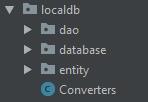
\includegraphics[width=0.6\linewidth]{images/LocalDB.png}
\caption{ Package local db}
\label{fig:pkgsharedata}
\end{figure}

\begin{enumerate}
\item Package dao: It contains interfaces that maps java function in SQL query.
\item Package database: this class contains the database abstract class.
\item Package entity: here classes that are mapped to the databases are present 
\end{enumerate}

\paragraph{Request}
In this paragraph the request package is presented. 
This package implements the client side of individual request service and group request service.

\begin{figure}[H]
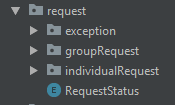
\includegraphics[width=0.6\linewidth]{images/Request.png}
\caption{ Package request }
\label{fig:pkgsharedata}
\end{figure}

\begin{enumerate}
\item Package exception: this contains the custom exceptions defined during the development.
\item Package individual request: here it is implemented the individual request user interface with fragments that can be loaded in the home
containers and the wrapper object that allows Object mapper to map immediately JSON strings to request objects. 
\item Package group request: same as above, but for group request. 
\end{enumerate}
	
\paragraph{Service}
In this package, the health service and the location service are implemented in order to receive data about health and position 
from, respectively, smartwatch or other similar devices and GPS. 
The application exploits the bluetooth functionality of the mobile device to receive the health data from the smartwatch, while for what 
concerns position data, it just receives it from the Location Manager of the device.\\

This package regards also AutomatedSOS and it is completely developed to work locally on the smartphone of the user. 

\begin{figure}[H]
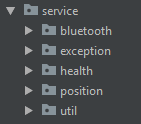
\includegraphics[width=0.6\linewidth]{images/Service.png}
\caption{ package service }
\label{fig:pkgsharedata}
\end{figure}

\begin{enumerate}
\item Package bluetooth: it contains a Bluetooth Server which is responsible of managing Bluetooth clients
\item Package exception: it contains all the custom exceptions used in the package
\item Package health: it contains the logic behind the health service which is based, basically, on the following: receiving the message;
saving the data if it is correct w.r.t. standard values; checking with simple threshold if the health is grave or not; if it is grave and
there are no recent emergency call, then it will get the user location and search for the emergency number within a JSON and call it
(afterwards, it saves the call on the local database to avoid flood calling)
\item Package util: it contains all the utilities class necessary for the health and position package. Here, it is important to  highlight the HealthDataInspectorImpl class in which it is defined the threshold of each field of health data:
\begin{itemize}
	\item heartbeat: the standard interval is $ [30, 220-age] $;
	\item minimum pressure: an interval of $ [40, 100]$;
	\item maximum pressure: an interval of $ [80, 200]$;
	\item blood oxygen level: it is a percentage of interval $ [80,100]$.
\end{itemize}
All these threshold are collected by an expert. If one of these thresholds are violated (excluded the case in which the health data is incorrect, i.e. bloody oxygen level not a percentage from 0 to 100), then the health data is considered to be grave and an emergency point should be called.
\item Package location: it contains the logic behind the location service, which just simply saves the position data on the local database
every time a new last location is present
\end{enumerate}

\paragraph{Share data}
Finally, the share data package is commented. 
The package structure is the same: it contains an exception package with the custom exceptions; it contains a network package with the
controller interface that exposes the function that allows the communication with share data service, and, finally, all the wrapper classes
for the mapping of the objects with JSON strings and vice versa.

\paragraph{Manifest folder}
This folder contains the application manifest that contains the properties of the application, like the definition of activities and user permission needed. 

\paragraph{Res folder}
Here are located all XML definitions files presented into the software. 
This files defines the aspect of the user interface and all the components styles.

\begin{figure}[H]
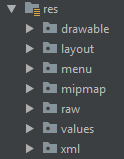
\includegraphics[width=0.6\linewidth]{images/Res.png}
\caption{ Res folder }
\label{fig:pkgsharedata}
\end{figure}

\begin{enumerate}
\item Package drawable: this package contains the XML definition of the drawable objects like images and icons.
\item Package layout: as the name says, it contains every activity layout. 
Note that the application is developed with automatically resizable layout and it supports portrait and landscape orientations.
\item Package menu: here there is the menu layout for the drawable menu on the left of the application.
\item Package mipmap: it contains the application icon.
\item Package raw: It contains two particular files. A JSON file with the last emergency call made by the user with Data4Help and keystore with the keys for secure communication.
\item Package value: here are stored string values, colors and component styles. 
\end{enumerate}



\section{Acceptance tests}
The approach to acceptance testing, for both data for help and automated SOS, has been
conducted in the following way. 
First of all, it has been decided to test all the possible use cases that are described in the
second version of the requirements and analysis document (of course, only the scenarios that
regards the implemented requirements and goals, mentioned in the implementation and document testing, have been considered). \\
The exceptions of the various use cases have been considered too, since the system should
behave properly, also, in these conditions. \\
Secondly, due to the fact that an user may behave in non-predicted way, other cases, for some
requirements have been considered. \\
Tests have been performed with JMeter. The source code is present in the delivery folder.

\par
The cases are presented in the next two subsections, each of which first exposes the
tests performed on the use cases divided by goal. After that, special cases and more strange
behaviours are considered. \\
Finally, at the end of this chapter, it is possible to find some brief conclusions. 

\subsection{Data for help tests}
\subsubsection{G1}
The uses cases that concerns G1 are: UC1, UC2, UC3, UC4, UC5, UC6, UC7 and UC9.  \\

\begin{itemize}
\item For what concerns UC1, the successful case has been tested (no exception is present), by using some requirements that involves the
third party registration and the possibility to send individual request. In particular, after having created a new third party customer,
and a new user; a request from that customer to the user is made. The user retrieves the list of pending requests (that contains only that
element) and approves and rejects it.

\item For testing UC2 a great number of third party customers has been created and registered: they all send a request to the same user.
The user retrieves all the pending requests and a check on the number of pending request: the behaviour is correct.
The exceptional case, requires the use of the front end: TODO

\item UC3 TODO

\item UC4 TODO

\item The test of UC5 has been performed togheter with UC1: after that the request is approved, we have checked that in the subscriptions
of the third party there exists one on a SSN that is equal to the user that accepted the request.

\item UC6 involves the sign up of user and individual requests. The successful case has been tested and also the cases in which SSN and email
are already present in the system. \\
The result is the following: userId and accessToken returned by the server are correct. In particular, they have been used to check
if the user was registered by performing an http request to retrieve the user's information.  \\
The exception about checking if fields are empty or not has been skipped since this is something that is implemented correctly in the front
end.

\item UC7 consists in logging users and third parties into the system. The normal event flow and the cases of wrong credential has been
tested.
The same check adopted in UC6 has been used here. \\ 
The exception that involves missing password or email, has been skipped since this is something that is implemented correctly in the front 
end.

\item UC9 TODO

\end{itemize}


\subsubsection{G2}
The uses cases that regards G2 are: UC6, UC7, UC8, UC9, UC32 and UC33.  \\


\begin{itemize}
\item The first two use cases (i.e. UC6 and UC7) were already presented above, while discussing G1.

\item To test UC8, basically, the idea is searching for the user SSN. 
If it is found it returns a bad request (i.e. this seems strange, but it is the correct chain-flow) with a specific message "Should send a
request to the individual to access his data". TODO COMMENT MORE ON THIS BEHAV.
After that, a request is sent: to check if things work properly, we have to be sure that the user has received a new pending request. 
The result is correct, but a the status of the HTTP request is 400 (i.e. bad request): in our opinion, this is not very good.  \\
The exceptions have been tested successfully. 
TODO CHECK IF WHAT WRITTEN IS CORRECT

\item UC9 TODO

\item UC32 and UC33 have not been implemented by the other team. TODO COMMENT ON WHAT YOU GET

\end{itemize}

\subsubsection{G3}
The uses cases that involves G3 are: UC6, UC7, UC11 and UC12.  \\

\begin{itemize}
\item 
As already mentioned, the first two use cases are just tested above during the test of G1.

\item 
During the test of UC11 is impossible to understand when there is an error message. 
In fact by doing the manual test, even 3 blocks of anonymized data are returned and no error message is shown. 
This is in conflict with what is expressed in the description of the use case of the RASD document. \\

TODO CHECK WHAT IS WRITTEN HERE: TOTALLY NO SENSE, USE SOME CONTEXT
For checking the creation of new data into the system just leave the server up. 
The more time the server is up, the more
data there are (i.e. every minute new data arrives), therefore we just check if the response is OK.

\item Since UC12 seems to equivalent to UC11, therefore the results are already discussed in the precedent point

\end{itemize}

\subsubsection{G4}
The uses cases that concerns G4 are: UC6, UC7, UC9, UC10, UC11, UC12, UC32, UC33 and UC34. \\

\begin{itemize}
\item 
UC6, UC7, UC9, UC11, UC12, UC33, UC32 are already discussed above

\item 
UC10 consists in the subscription of a third party customer to new user data. \\
In the website, the subscribe is done when a checkbox is crossed during the search of bulk data. 
While testing with JMeter, the search has been skipped and only an HTTP request to directly subscribe has been done.
To check if things work properly, the subscriptions of that third party are retrieved: since the subscription id is present, the
result is correct.

\item UC31 has not been implemented by the other team. TODO DESCRIBE THE BEHAV.

\end{itemize}

\subsubsection{Other tests}
TODO ALL (if you are going to test only with the front end, please, change the description of the structure mentioned above) 
\subsection{Automated SOS tests}
Mystery of faith!!
\subsection{Conclusion}
The prototype has been developed until a good point, but it still contains some bugs. In particular, many of them regards the user interface
and the website. \\
For what concerns the single goals, we can say the following:

\begin{itemize}
\item
It is possible to state that G1 has been reached. However there are some problems with the notification of third party when individual
requests are approved or rejected.

\item
A same reasoning can be applied also to G2. Indeed, UC32 and UC33 present problems with the notifications

\item
G3 has not been fully reached. To be precise, there is the problem with the constraint on 1000 individuals while accessing bulk data

\item 
G4 is achieved correctly

\item 
For what concerns G5, it has been possible to test graphically only the fact that, after having registered a user older than 60 years old, 
and when 10 seconds are elapsed, a request arrives from ASOS, that is some kind of special third party customer. \\
As mentioned in the section regarding the test of G5, the other functionalities could not be tested.\\

\par
In conclusion, the prototype is not ready to be deployed on the market due to previous problems.

\end{itemize}




\section{Installation instruction}
\subsection{Microservices}
First of all, let's check all the prerequisites needed to install and run the software:

\begin{itemize}

\item RabbitMQ is necessary, since a RabbitMQ server is needed to make the communication between microservices properly working.
It is possible to download it from there: \url{https://www.rabbitmq.com/download.html}. \\
Once the page is opened, click on the links on the right, selecting the right operative system and download the installer. 
When working with windows, it may be possible that the installation process throws an error that expresses the necessity of downloading
the Erlang programming language. In this case, just follow \url{http://www.erlang.org/downloads} and download Erlang for the version
of Windows that you are using

\item MySQL is another critical component since it has been used as a DBMS for managing persistent data. For having this working, it
is possible to follow the guide at : \url{https://beep.metid.polimi.it/documents/121843524/b5d81926-98f6-496f-bf45-a2a8e897228c} 
(ignore all the chapter regarding NetBeans and follow the ones that deal with the installation of MySQL). \\
Once that the server has been set up, it is necessary to create the databases and its admin: to do that, first of all, go to the MySQL 
folder and login with root. After that, write:
 \begin{verbatim}
create user 'trackmeadmin'@'%' identified by 'datecallmeeting95';
\end{verbatim}
Now, the admin for the database has been created, and it is necessary to create all the databases used by the various microservices. \\
In order to accomplish this, run:
\begin{verbatim}
create database share_data_db;
create database group_request_db; 
create database individual_request_db;
create database account_service_db;
\end{verbatim}
Finally, for each database created, it is necessary to run this command: 
\begin{verbatim}
grant all on db_name.* to 'trackmeadmin'@'%';
\end{verbatim}
where db\_name has to be substituted with share\_data\_db, group\_request\_db, account\_service\_db and individual\_request\_db. 

\end{itemize}

Once that all the previous steps have been accomplished, and once you have downloaded all the jars from the links present in the front page
of this document, start MySQL server (following the guide mentioned above), and after that start the RabbitMQ server. In order to do that, 
navigate to that folder in which RabbitMQ have been installed, search for "rabbitmq-server" and launch it (if you prefer other ways to launch
the server you may check the link provided before: indeed, the links to the installation instruction of the various operative systems,
provide also information on how to set up the server). \\
After that, it is possible to start the downloaded jars by means of: 
\begin{verbatim}
java -jar path/to/file.jar
\end{verbatim}
It is necessary to start first of the service registry, and then all the other services (and, of course, also the API gateway), in the
order you prefer. 
The port that are needed to be free are the following: 8443 (API gateway), 8761 (service registry), 8089 (share data service), 8081 (group
request service), 8082 (individual request service). However, if for some reasons one of these ports is busy on the
machine in which the jar will be ran, it is possible to modify the port by adding "--server.port=PORT\_NUMBER", while launching the jar. Moreover, to expose the server to the mobile application it is important to change the server address with the local IP of the machine by adding to the api gateway jar launch "--server.address=LOCAL\_IP" \\
Furthermore, is also possible to modify any of the settings that are located within the application.properties of the various project.
One can find these files in the various folders of the source code, within the folder "main". However, in order to avoid useless errors
we suggest to not modify critical parts, such as the routes used by Zuul (API gateway settings). \\

\par 
For running the tests, it is necessary to start again the RabbitMQ server and the MySQL server. After that, it is possible to go into
the root of interested project and run "mvn test". \\
Keep in mind that running the tests may take some time, due to the fact that some tests require to launch the entire spring application,
or to connect to the RabbitMQ server, or to load data into the database. In case there has been some errors due to integration 
tests with RabbitMQ, it can help to open the web server of RabbitMQ: localhost:15762, enter as guest with the password "guest" 
and purge the queues if necessary.

\par 
Here it follows a list of further considerations: 
\begin{itemize}
\item If, for some reason, it is necessary to open the source code in some IDE, keep in mind that it
may be necessary to download the Lombok plugin. \\
In the case in which you are using Intellij, this link may be useful:\\
\url{https://projectlombok.org/setup/intellij}

\item Another thing that one may take into consideration, is the fact that when downloading the source code, one may have problem with too long
paths when extracting the folder. This is a problem that have been encountered only extracting the zip, and that is fixed
by using tar.gz format. 

\item When running tests that are provided with the source code, remember to not having started the application as a whole, or at least not
the one that involves the test that is going to start. This is because the same service which is running could steal the messages from the test execution environment and, therefore, conflicts can happen, leading to some bugs. \\
Furthermore, there is a timeout set to 1 minute, regarding the exchange of messages in the message queue. Keep in mind that you are probably
running an entire architecture on a single machine, therefore don't get surprised if things get stuck a bit. However, we didn't encountered
many problems in this sense.

\item If you are opening the source code in your IDE (e.g. IntelliJ) and you run the program from there, you should also configure
the databases inside the IDE. In this sense, since all the microservices are different projects, it is necessary to link each database
to its related project. \\ A final remark is that the account service db is related to the API gateway; for what concerns the others, instead,
the binding is trivial.   

\item Due to setting of the application.properties file, every time that a jar is launched the database will be created and therefore
it will need to be re-populated. A little exception holds for what concerns the API gateway: indeed a SQL script named "data.sql" will be
executed loading a table that contains information regarding the available API. \\ 
If there is the necessity to avoid creation of a new database, then when launching the jar it is possible to add "--spring.jpa.hibernate.ddl-auto=update" to set the hibernate to update mode.

\item 
\end{itemize}

\par
In order to run the test plans of JMeter it is necessary to have JMeter installed. Then since RabbitMQ queues has to be purged and the DBs has to be deleted, it is necessary to add some libraries:
\begin{itemize}
\item mysql-connector.jar (\url{https://dev.mysql.com/downloads/connector/j/}) to be moved into the lib folder of JMeter
\item amqp-client-3.x.x.jar (\url{https://www.rabbitmq.com/java-client.html} to be moved into the lib folder of JMeter; remember to download a version starting with 3, e.g. 3.6.6 (\url{http://repo1.maven.org/maven2/com/rabbitmq/amqp-client/})
\item Download also the project \url{https://github.com/jlavallee/JMeter-Rabbit-AMQP} and build it with Ant ("brew install ant" for Mac users). Then move the generated jar file, which can be found in /target/dist, into the lib/ext folder of JMeter. To avoid searching for this jar, it is possible to download it directly on the release section of GitHub
\end{itemize}
After this configuration, it is possible to run the test plans of JMeter on GUI/non-GUI mode: 
\begin{itemize}
	\item GUI Mode: to launch this mode, just double-click on the jmeter executable or launch it with the terminal; in order to run the test, it is possible to just click on the green play button on the top bar. After that it is possible to see the results by clicking on the node: "View Results Tree" or "View Results on Table" located in every thread group
	\item non-GUI Mode: To launch this mode, just run this code on the terminal: "jmeter -n -t [jmx file] -l [results file] -e -o [Path to web report folder]" which will output a result file of the test and a html web page report on the folder chosen where there will be graphic representation of the results of the test. If the command does not work properly it is possible to run the code separately: first "jmeter -n -t [jmx file] -l [results file]" and then run "jmeter -g [results file] -o [Path to web report folder]".
\end{itemize}
In case the api-gateway service is running on a IP different from localhost, then it is necessary to change the IP address of the test from the GUI: just click on the HTTP 
request default that can be found on the left side of the graphical interface and change the IP address with the one chosen.

\subsection{Android application}
In order to install the application onto your device it is necessary to allow the installation of applications from unknown sources. This setting can be found in your device's system settings under: Settings > Applications > Unknown sources. 
\\
Now it is possible to download the apk from the project folder on GitHub and after that, it is possible to install it by launching the Downloads application. The Downloads application can be launched from web browser using the menu, or by launching the 
Downloads applications directly by the download folder on your device. During the first launch of the application the user must 
accept all the permission required. Note that if some are refused then the application will be closed. For the first execution the 
user should set the ip address of the server by pressing on the TrackMe logo in the user login. A window with the current ip 
address is shown and here it is possible to change the address with the one of the machine in which you are running the jars. 
For simulating the smartwatch it is also necessary to download the bluetooth client APK from the GitHub folder and install it, by following the same instruction reported above.

\par 
Here it follows a list of further considerations: 
\begin{itemize}
\item If, for some reason, it is necessary to open the source code it may be necessary to download Android Studio and set up the emulator. \\
\end{itemize}

\par
If the reader does not have a mobile phone with android he can use an emulator on his pc, but the bluetooth connection cannot be simulated with an emulator.

Regarding the tests of the health service, all the tests should be launched on an android simulator with some tweak configurations to do:
\begin{itemize}
\item Enable the developer settings by tapping a lot of time on the build settings of the simulator.
\item Enable the mock position for the application through the developer settings.
\end{itemize}
Moreover, the test regarding the bluetooth does not exist due to complexity: the simulator does not have the capacity to 
simulate bluetooth connections. Instead, there is a stub application bluetooth client which can be used to test if the 
communication between bluetooth devices is working as expected. Therefore, it is necessary to have two devices 
supporting bluetooth which are paired. Then after starting the health service on the device containing TrackMe application, 
a bluetooth server is running in background waiting for other devices. Now after starting the other application, it should be possible 
to insert the name of the device running the server and establish the connection. Once the connection is established it is possible 
to simulate the sending operation of health data; to test the call procedure of the emergency point it is necessary to send a health 
data which is grave (i.e. one of the threshold is violated). After sending the data, the main phone running TrackMe application 
should make a call to a number where the suffix of the number is 118 if in Italy (due to testing reason, it was not possible to truly 
call the emergency point since this is a prototype application).
Since the bluetooth client application is just a stub, it is not so user friendly, therefore, it can be seen that the connection is active 
only when the send data button is active, otherwise if it is not, check if the devices are paired and the bluetooth server is activated or 
just retry to connect.




\newpage

\begin{thebibliography}{9}

\bibitem{androidELS}
Android emergency location service, URL \url{https://crisisresponse.google/emergencylocationservice/how-it-works/}

\bibitem{httpstool}
Working with certificates and SSL, URL \url{https://docs.oracle.com/cd/E19830-01/819-4712/ablqw/index.html}

\bibitem{spring}
Spring framework, URL \url{https://spring.io}

\bibitem{rabbitMQ}
RabbitMQ, URL \url{https://www.rabbitmq.com}

\bibitem{rabbit-concepts}
RabbitMQ concepts about exchanges and queues, URL \url{https://www.rabbitmq.com/tutorials/amqp-concepts.html}

\end{thebibliography}

\end{document}
